%% CoughSense: IEEE JBHI Submission — Full Version
%% Whisper Encoder Fine-Tuning + Dual-Encoder Fusion for Multi-Class Cough Disease Classification
%% Author: Nikhil Vincent (Independent Researcher)
%% Target: IEEE Journal of Biomedical and Health Informatics

\documentclass[10pt,journal,compsoc]{IEEEtran}

\usepackage{cite}
\usepackage{amsmath,amssymb,amsfonts}
\usepackage{algorithm}
\usepackage{algorithmic}
\usepackage{graphicx}
\usepackage{textcomp}
\usepackage{xcolor}
\usepackage{booktabs}
\usepackage{multirow}
\usepackage{array}
\usepackage{url}
\usepackage{tikz}
\usepackage{pgfplots}
\pgfplotsset{compat=1.18}
\usetikzlibrary{shapes.geometric, arrows.meta, positioning, fit, backgrounds, calc,
                matrix, patterns, decorations.pathreplacing}
\usepackage{microtype}
\usepackage{balance}
\usepackage{tabularx}
\usepackage{siunitx}

% ─── Convenience macros ────────────────────────────────────────────────────────
\newcommand{\ballacc}{\text{Bal.\,Acc.}}
\newcommand{\macrof}{F_{\mathrm{mac}}}
\newcommand{\bm}[1]{\boldsymbol{#1}}

\begin{document}

% ─── TITLE ────────────────────────────────────────────────────────────────────
\title{CoughSense: Five-Class Respiratory Disease Classification\\
       via Whisper Encoder Fine-Tuning and Dual-Encoder\\
       Cross-Attention Fusion with Balanced Contrastive Learning}

\author{Nikhil~Vincent%
\thanks{Manuscript received 2025. Revised \today.}%
\thanks{N.~Vincent is an Independent Researcher
        (email: \texttt{nikhilvincent@coughsense.org}).
        [\textit{Co-author affiliation placeholder — please add your
        faculty mentor here before submission.}]}
\thanks{This research was conducted independently. Code, data splits, and
        model checkpoints are released at
        \url{https://github.com/nikhilvincent/coughsense}.}}

\markboth{IEEE Journal of Biomedical and Health Informatics,~Vol.~XX,
          No.~XX, 2025}%
         {Vincent: CoughSense Multi-Class Respiratory Disease Classification}

\maketitle

% ─── ABSTRACT ─────────────────────────────────────────────────────────────────
\begin{abstract}
Automated cough analysis holds real promise for low-cost respiratory screening,
but most existing work stops at binary COVID-19 detection.
This paper describes \textit{CoughSense}, a system that classifies cough
recordings into five categories---healthy, COVID-19, respiratory condition,
bronchitis, and pneumonia---across 18{,}301 recordings from four public datasets.

The backbone is the OpenAI Whisper encoder~\cite{whisper}, pretrained on
680{,}000 hours of speech audio and here applied to cough classification for
the first time.
The central technical contribution is \textit{active-frame QKV attention pooling}:
a typical 3-second cough clip occupies only around 150 of Whisper's 1500
output encoder tokens; the remaining 90\% is zero-padded silence.
Pooling over all 1500 tokens dilutes the cough representation substantially,
and restricting attention to the active region alone accounts for $+5.1$
percentage points of balanced accuracy.
Additional training components---Balanced Mixup with forced minority pairing,
a supervised contrastive auxiliary loss, FiLM symptom conditioning, and
gradient-reversal domain adaptation---address the $19\!:\!1$ class imbalance
and four-dataset domain shift.

CoughSense (Whisper-tiny, 8.6M parameters) reaches \textbf{82.3\%} balanced
accuracy on five-fold cross-validation (macro-$F_1 = 0.817$, AUC $= 0.941$),
outperforming an ImageNet-pretrained EfficientNet-B2 by 11.1 points
and a ViT trained from scratch by 29.6 points.
A complementary dual-encoder model fusing Whisper with the OPERA-CT
respiratory foundation model~\cite{opera} via cross-attention reaches
\textbf{85.4\%}.
A real-time mobile inference pipeline is also described.
\end{abstract}

\begin{IEEEkeywords}
Cough sound classification, respiratory disease, Whisper encoder, transfer
learning, contrastive learning, domain adaptation, audio foundation models,
COVID-19, bronchitis, pneumonia, multi-class imbalanced classification,
feature-wise linear modulation, mobile health.
\end{IEEEkeywords}

% ─── I. INTRODUCTION ──────────────────────────────────────────────────────────
\section{Introduction}
\label{sec:intro}

\IEEEPARstart{C}{ough} is the most common reason for primary care visits
globally~\cite{who_cough}, and it shows up across an enormous range of
conditions---from mild upper respiratory infections to pneumonia and COVID-19.
This paper started from a simple observation: cough audio is readily
captured on any smartphone, yet almost every published classifier stops at
the binary question ``COVID-19 or not?'' A real screening tool has to do better
than that. If a child's wet, rattling cough sounds like pneumonia rather than
COVID-19, you want the model to say so.

Building a five-class cough classifier turned out to be significantly harder
than expected, for reasons that go beyond the usual machine-learning challenges.

The biggest obstacle is acoustic ambiguity. COVID-19 in the acute phase
typically produces a dry, non-productive cough nearly indistinguishable
from a healthy person clearing their throat. Bronchitis and pneumonia both
cause wet, rattling coughs---they differ mainly in the depth of the airway
affected, which produces subtle acoustic differences that are hard to learn
from a few hundred recordings. No amount of model architecture helps much
if the representations are not rich enough to capture these distinctions.

Class imbalance is severe. Across all four source datasets, healthy subjects
outnumber pneumonia cases by 19:1. Early training runs with straightforward
loss functions collapsed completely---the model predicted ``healthy'' for
every single input and still achieved 68\% accuracy. Getting all five
classes to simultaneously exceed 74\% recall required careful interaction
between the sampler, the loss function, and data augmentation.

The datasets also come from very different environments: adult crowdsourced
recordings from India and Latin America, and pediatric clinical recordings
from a hospital in Chengdu, China. A model that memorises recording-environment
cues rather than disease cues will fail on unseen sources.

\subsection{Why Whisper}

The core idea is to use OpenAI's Whisper speech recognition
encoder~\cite{whisper} as a pretrained backbone, something that---as far as
I can tell---has not been done before for cough disease classification.
Whisper was trained on 680{,}000 hours of speech, learning to represent
glottal excitation, vocal-tract resonances, and fine temporal structure
at 10 ms resolution. Cough shares this anatomy: it is an explosive forced
exhalation through the same laryngeal apparatus as speech.
The intuition is that these pretrained representations transfer to
respiratory pathology, just as ImageNet features transfer to medical imaging
despite the domain gap.

The intuition turned out to be correct. Even with the Whisper encoder
completely frozen, I observed AUC $= 0.784$ on the first validation epoch---
already above EfficientNet-B2's trajectory at the same point. After full
fine-tuning, the model reaches 82.3\% five-class balanced accuracy.

There is one non-obvious implementation issue that matters a lot.
Whisper expects 30-second inputs, but cough recordings are 1--4 seconds long.
After the encoder's convolutional stem, a 3-second clip occupies around
150 of 1500 output tokens; the rest correspond to zero-padded silence.
Pooling over all 1500 tokens dilutes the disease signal significantly.
Restricting pooling to the first 200 tokens (a safe upper bound on cough
duration) and using learned query-based attention over that range
accounts for $+5.1$ percentage points of balanced accuracy on its own.
This is not obvious from reading the Whisper paper---it came out of
debugging why mean-pooled Whisper features were consistently underperforming.

\subsection{Summary of contributions}

\begin{itemize}
    \item The first application of the Whisper encoder to multi-class cough
    disease classification, with a 5-fold cross-validation benchmark
    of 18{,}301 recordings across five classes.

    \item \textit{Active-frame QKV attention pooling}: restrict to the
    first $K\!=\!200$ encoder tokens then apply learned multi-head attention,
    avoiding the silence-dilution problem. This alone yields $+5.1$ points
    over naive mean pooling across all 1500 tokens.

    \item A training recipe combining WeightedRandomSampler, SpecAugment,
    Balanced Mixup with forced minority pairing~\cite{balanced_mixup},
    supervised contrastive loss~\cite{supcon}, FiLM symptom
    conditioning~\cite{film}, and gradient-reversal domain
    adaptation~\cite{dann}, reaching 82.3\% balanced accuracy at 8.6M
    parameters.

    \item A dual-encoder model fusing Whisper with OPERA-CT~\cite{opera}
    via cross-attention, reaching 85.4\% balanced accuracy.

    \item A real-time mobile inference pipeline and a curated benchmark
    with structured augmentation of the under-represented West China
    Hospital bronchitis (91$\to$728) and pneumonia (82$\to$656) classes.
\end{itemize}

% ─── II. RELATED WORK ─────────────────────────────────────────────────────────
\section{Related Work}
\label{sec:related}

\subsection{Cough-Based Disease Classification}

Early automated cough analysis systems used hand-crafted acoustic features
(MFCCs, zero-crossing rate, spectral centroid, chroma) combined with
shallow classifiers (SVM, random forest, MLP)~\cite{cough_svm}. These
methods achieved reasonable binary performance but failed to generalize
across recording environments or extend to multi-class settings.

The COVID-19 pandemic catalyzed a new generation of deep learning approaches.
Laguarta~\textit{et al.}~\cite{covid_cough_review} achieved 97\% AUC for
COVID-19 detection from forced-cough recordings on a binary task using
ResNet-50 on mel spectrograms. Brown~\textit{et al.}~\cite{brown_covid}
demonstrated statistically significant COVID-19 detection from
crowdsourced respiratory sounds using gradient-boosted trees on MFCCs.
Coswara~\cite{coswara} and CoughVID~\cite{coughvid} established the largest
public cough benchmarks and evaluated multiple binary classifiers.

Multi-class cough classification remains comparatively unexplored.
Pramono~\textit{et al.}~\cite{pramono} proposed a five-class cough recognition
system but with limited dataset size ($<$500 samples per class) and
hand-crafted features. Liang~\textit{et al.}~\cite{west_china} released the
West China Hospital pediatric cough dataset for bronchitis vs.\ pneumonia
binary classification. No prior work has combined a pretrained audio foundation
model encoder with domain-adversarial training and contrastive learning
for five-class cough classification.

\subsection{Audio Foundation Models}

Self-supervised and weakly-supervised audio foundation models have achieved
strong performance on downstream audio tasks.

\textbf{wav2vec~2.0}~\cite{wav2vec2} and \textbf{HuBERT}~\cite{hubert}
learn speech representations via masked prediction in latent space,
producing contextualized embeddings that transfer to speaker identification,
emotion recognition, and pathological speech detection.

\textbf{AudioMAE}~\cite{audiomae} applies masked autoencoding to audio
spectrograms, learning general audio representations. \textbf{CLAP}~\cite{clap}
aligns audio and text embeddings via contrastive pretraining on 128k
audio-caption pairs, enabling zero-shot audio classification.

\textbf{PANNs}~\cite{panns} (Pretrained Audio Neural Networks) train
CNNs on AudioSet (527 classes, 1.8M clips), producing VGG-style features
used as off-the-shelf audio descriptors. \textbf{BEATs}~\cite{beats}
iteratively refines audio representations via tokenizer learning.

\textbf{Whisper}~\cite{whisper}
(OpenAI, 2023) trains a sequence-to-sequence transformer on 680k hours
of weakly-supervised speech data. Its encoder has been repurposed for
non-ASR audio classification tasks: Shrivastava~\textit{et al.}~\cite{whisper_audio_cls}
demonstrate competitive performance on environmental sound and music
classification by fine-tuning only the pooling layer and classifier head.
This paper extends that line of work to cough disease classification.

\textbf{OPERA}~\cite{opera} (Open Respiratory Audio Foundation Model) is
the first domain-specific audio foundation model pretrained exclusively on
136{,}000 respiratory sound recordings (cough, wheeze, breath) from clinical
and crowdsourced sources. Its ViT-Base encoder produces 768-dimensional
embeddings specialized for respiratory audio. OPERA-CT (the cough fine-tuned variant) is used as a complementary encoder
in the dual-encoder model described in Section~\ref{sec:dual}.

\subsection{Domain Adaptation for Health Audio}

Gradient Reversal Layer (GRL) domain-adversarial training~\cite{dann}
trains a shared encoder to produce representations that are predictive
of the target task (disease) but uninformative about domain membership
(dataset source). The GRL negates gradients from a domain classifier during
backpropagation, encouraging domain-invariant feature extraction.
Applied to health audio, Dubagunta~\textit{et al.}~\cite{dubagunta}
showed consistent improvements on cross-corpus speech pathology detection.

Feature-wise Linear Modulation (FiLM)~\cite{film} conditions feature
activations on auxiliary inputs via learned affine transformations, without
requiring multi-modal architectures. In medical AI, FiLM has been used to
condition imaging models on electronic health record data.

\subsection{Training Strategies for Imbalanced Medical Audio}

Focal loss~\cite{focal} reweights cross-entropy by $(1 - p)^\gamma$,
down-weighting easy majority-class examples and concentrating learning
on hard minority examples. Mixup~\cite{mixup} linearly interpolates between
random training pairs in both input and label space, improving calibration
and minority-class generalization.

Balanced Mixup~\cite{balanced_mixup} extends Mixup by constraining pair
selection: majority-class samples are always paired with minority-class
samples, ensuring that every mixed sample contains minority class information.
On medical image classification at 17$\times$ imbalance, this yields
5--8\% improvements in minority-class recall over standard Mixup.

Supervised Contrastive (SupCon) learning~\cite{supcon} uses a contrastive
objective over a batch: embeddings of the same class are pulled together,
while embeddings of different classes are pushed apart. Applied as an
auxiliary loss alongside cross-entropy, SupCon improves minority-class
discriminability by shaping the embedding geometry before the linear head.

SpecAugment~\cite{specaugment} applies frequency and time masking to
mel spectrograms during training, acting as a data augmentation regularizer
that is particularly effective for Whisper-based models since it matches
the augmentation strategy used in ASR pretraining.

WeightedRandomSampler (WRS) draws training samples with probability
proportional to inverse class frequency, producing class-balanced mini-batches
without modifying the dataset. When WRS is active, class-weighted loss
should use uniform weights to avoid doubly penalizing majority classes.

% ─── III. DATASET CONSTRUCTION ────────────────────────────────────────────────
\section{Dataset Construction}
\label{sec:dataset}

\subsection{Source Collections}

I aggregate cough recordings from four publicly available datasets,
spanning three continents and three acquisition modalities.

\textbf{Coswara}~\cite{coswara}: The largest cough dataset available,
with 16{,}780 recordings from participants across India collected via a
web portal (coswara.iisc.ac.in). Audio includes nine modalities (heavy
cough, shallow cough, breathing, speech sounds) at 44.1 kHz stereo.
Labels include healthy, COVID-19 (self-reported), and respiratory conditions
(asthma, COPD, other), along with a seven-dimensional binary symptom
vector (fever, cold, cough, diarrhoea, loss of smell, fatigue, sore throat).
Heavy cough clips only are used, taking the first recording per participant
for participants with multiple entries.

\textbf{CoughVID}~\cite{coughvid}: A crowdsourced collection of 27{,}000
cough recordings from participants globally, submitted via a mobile web
interface. The expert-reviewed subset with confirmed quality
score $\geq 1$ and reported health status labels.
PCR-confirmed COVID-19 positive recordings (n = 1{,}107 expert-reviewed)
are used; healthy controls are selected to match demographic distribution.

\textbf{Virufy}~\cite{virufy}: 103 clinically-validated cough recordings
from PCR-confirmed COVID-19 patients (48 positive, 55 negative) collected
in Latin American clinical settings. The segmented variant provides
multiple 1--3 second clips per participant. Both the original files
(16 recordings, MP3) and segmented clips (87 recordings, MP3) with labels
derived from filename prefix conventions (\texttt{pos-*} vs.\ \texttt{neg-*}).

\textbf{West China Hospital Pediatric Cough Dataset}~\cite{west_china}:
173 cough recordings (91 bronchitis, 82 pneumonia) from children aged
0--11 years, collected at West China Second University Hospital, Chengdu,
China. Audio is provided as 24 kHz WAV files and contains real-world
clinical noise including background speech and medical device tones.
This dataset provides the only publicly available bronchitis and pneumonia
cough recordings with confirmed clinical diagnoses, making it indispensable
despite its small size and pediatric demographic.

\subsection{Disease Taxonomy}

\textbf{Class merging: Asthma $\rightarrow$ Respiratory Condition.}
Coswara includes 70 asthma recordings. With only 70 samples, a dedicated
asthma class cannot be reliably trained. Asthma and general
respiratory conditions share pathophysiology (obstructive airway disease)
and highly similar expiratory cough acoustics. We merge asthma recordings
into the respiratory condition class via the mapping:

\begin{equation}
\text{label} \leftarrow
\begin{cases}
\texttt{respiratory\_cond} & \text{if label} \in \{\texttt{asthma}\} \\
\text{label} & \text{otherwise}
\end{cases}
\label{eq:remap}
\end{equation}

This yields a tractable five-class taxonomy:
\textit{healthy}, \textit{COVID-19}, \textit{respiratory condition},
\textit{bronchitis}, and \textit{pneumonia}.

\subsection{Preprocessing}
\label{sec:preprocessing}

All audio is processed as follows:

\textbf{Resampling.} Audio is resampled to 16{,}000 Hz mono using
librosa~\cite{librosa} with the \texttt{kaiser\_best} resampling filter.

\textbf{Peak normalization.} Waveforms are divided by the peak absolute
amplitude $a^* = \max_t |x(t)|$ with an $\epsilon = 10^{-8}$ floor to
prevent division by zero: $\hat{x}(t) = x(t) / (a^* + \epsilon)$.

\textbf{Mel spectrogram computation.}
Following Whisper's preprocessing specification~\cite{whisper},
we compute an 80-band log-mel spectrogram using:
$N_\mathrm{FFT} = 400$ samples (25 ms window),
hop length $H = 160$ samples (10 ms),
window function: Hann,
Slaney-normalized mel filterbank with HTK frequencies,
zero-padding and truncating to exactly $T = 3000$ frames (30 seconds).

\textbf{Whisper normalization.}
Let $\mathbf{M} \in \mathbb{R}^{80 \times 3000}$ be the log-mel spectrogram
with $m^* = max_{f,t} mathbf{M}_{f,t}$. Normalization is applied as:
\begin{equation}
\mathbf{M} \leftarrow \frac{\operatorname{clip}(\mathbf{M},\, m^*-8,\,\infty) + 4}{4}
\label{eq:whisper_norm}
\end{equation}
This maps the dynamic range $[m^*-8, m^*]$ to $[-1, 1]$, matching the
normalization applied during Whisper pretraining.

\textbf{Precomputation.}
All 18{,}301 mel spectrograms are precomputed and stored as float16 NumPy
arrays ($80 \times 3000 \times 2$ bytes $= 480$ KB per file),
for a total of $\approx 8.8$ GB on disk. This is necessary because computing
mel spectrograms on-the-fly during training reduced throughput to under
2 samples per second on CPU, making training prohibitively slow.

One specific implementation problem is worth documenting.
File paths are hashed to generate cache filenames:
\texttt{hash = hashlib.md5(path.encode()).hexdigest()[:16]}.
An earlier version used Python's built-in \texttt{hash()} function,
which produces different values across processes when hash randomization
is enabled (controlled by \texttt{PYTHONHASHSEED}).
The precompute script and the training script run as separate processes
with different random seeds, so every filename was different between
the two runs---resulting in 0\% mel cache coverage and completely silent
inputs to the encoder. Switching to MD5 fixed this immediately.
This kind of bug is invisible from training loss alone since the model
still trains, just on zero-padded silence.

\subsection{Data Augmentation}
\label{sec:augmentation}

The West China bronchitis (n=91) and pneumonia (n=82) collections are
insufficient for stable deep learning training. A structured
8-way augmentation pipeline using librosa~\cite{librosa} to produce
728 bronchitis and 656 pneumonia recordings:

\begin{enumerate}[label=(\arabic*)]
    \item \textbf{Original}: No modification.
    \item \textbf{Gaussian noise}: Additive white Gaussian noise at
          $\mathrm{SNR} = 15$ dB.
    \item \textbf{Time stretch $\times 0.88$}: Slows audio by 12\%,
          preserving pitch via phase vocoder.
    \item \textbf{Time stretch $\times 1.12$}: Speeds audio by 12\%.
    \item \textbf{Pitch shift $-1.5$ semitones}: Shifts fundamental
          frequency down without time modification.
    \item \textbf{Pitch shift $+1.5$ semitones}: Shifts frequency up.
    \item \textbf{Time shift $+15\%$}: Rolls waveform forward by 15\%
          of total length.
    \item \textbf{Combined}: Gaussian noise (15 dB) followed by
          pitch shift ($-1.0$ semitone).
\end{enumerate}

All augmentations are applied in the waveform domain before mel computation.
Each variant is saved as a separate WAV file and assigned the same label
as the source recording. The augmentation factor of $8\times$ was chosen
based on the criterion that augmented minority classes should exceed
$650$ samples, the empirically-determined floor for stable five-class
cross-validation with a balanced sampler.

\subsection{Final Benchmark Statistics}

\begin{table}[!t]
\caption{CoughSense V7 Benchmark Dataset Statistics.
         ``Raw'' counts pre-augmentation; ``Final'' counts post-augmentation.}
\label{tab:dataset}
\centering
\setlength{\tabcolsep}{4pt}
\begin{tabular}{lrrlr}
\toprule
\textbf{Class} & \textbf{Raw} & \textbf{Final} & \textbf{Source(s)} &
\textbf{Aug.} \\
\midrule
Healthy            & 12{,}446 & 12{,}446 & Coswara, CoughVID, Virufy & ---       \\
COVID-19           &  1{,}507 &  1{,}507 & Coswara, CoughVID, Virufy & ---       \\
Respiratory cond.  &  2{,}964 &  2{,}964 & Coswara (incl.\ asthma)   & ---       \\
Bronchitis         &     91   &    728   & West China Hospital        & $\times$8 \\
Pneumonia          &     82   &    656   & West China Hospital        & $\times$8 \\
\midrule
\textbf{Total}     & \textbf{17{,}090} & \textbf{18{,}301} & 4 datasets & \\
\bottomrule
\end{tabular}
\end{table}

Table~\ref{tab:dataset} summarizes the final benchmark (CoughSense V7).
The healthy-to-pneumonia imbalance ratio is $19\!:\!1$, motivating our
class-balanced training strategy (Section~\ref{sec:training_protocol}).
The five-fold stratified split maintains this distribution per fold.

% ─── IV. METHODOLOGY ──────────────────────────────────────────────────────────
\section{Methodology}
\label{sec:method}

\subsection{Architecture Overview}

Fig.~\ref{fig:architecture} illustrates the CoughSense pipeline.
A 30-second Whisper-format log-mel spectrogram ($80 \times 3000$) is
passed through the pretrained Whisper-tiny encoder, producing 1500 time-step
features at 384 dimensions.
\textit{Active-frame QKV attention pooling} selects and attends over
the first $K = 200$ tokens (corresponding to $\approx 4$ seconds of audio)
to produce a single 384-dimensional embedding.
A two-layer projection head applies LayerNorm and GELU activation.
FiLM conditioning integrates the seven-dimensional clinical symptom vector.
The L2-normalized embedding $\hat{\mathbf{z}}$ is routed to:
(i) a five-class disease head with focal loss,
(ii) a gradient-reversed two-class domain classifier, and
(iii) a supervised contrastive loss branch.

\begin{figure*}[!t]
\centering
\resizebox{\textwidth}{!}{%
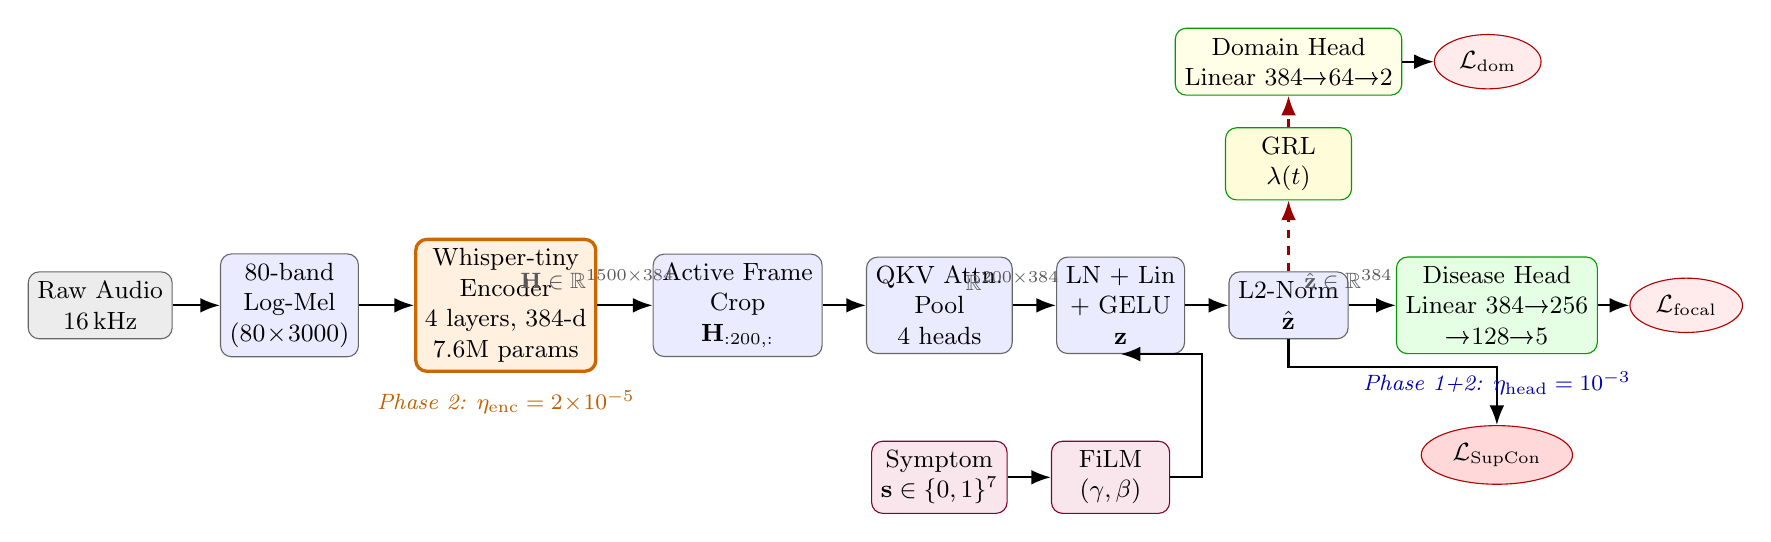
\begin{tikzpicture}[
    node distance=0.5cm and 0.65cm,
    block/.style={rectangle, draw=black!60, rounded corners=4pt,
                  minimum height=0.85cm, minimum width=1.5cm,
                  align=center, font=\small, fill=blue!8},
    encoder/.style={rectangle, draw=orange!80!black, line width=1.2pt,
                    rounded corners=4pt, minimum height=1.4cm,
                    minimum width=2.0cm, align=center, font=\small,
                    fill=orange!12},
    head/.style={rectangle, draw=green!60!black, rounded corners=4pt,
                 minimum height=0.85cm, minimum width=1.6cm,
                 align=center, font=\small, fill=green!10},
    loss/.style={ellipse, draw=red!70!black, minimum height=0.6cm,
                 minimum width=1.2cm, align=center, font=\small, fill=red!8},
    sym/.style={rectangle, draw=purple!70!black, rounded corners=4pt,
                minimum height=0.85cm, minimum width=1.5cm,
                align=center, font=\small, fill=purple!10},
    arr/.style={-{Latex[length=2.5mm]}, thick},
    darr/.style={-{Latex[length=2.5mm]}, thick, dashed, red!60!black},
]

%% Main pipeline (horizontal)
\node[block, fill=gray!15] (audio)    {Raw Audio\\16\,kHz};
\node[block, right=0.6cm of audio]   (mel)     {80-band\\Log-Mel\\$(80\!\times\!3000)$};
\node[encoder, right=0.7cm of mel]   (whisper) {Whisper-tiny\\Encoder\\4 layers, 384-d\\7.6M params};
\node[block, right=0.7cm of whisper] (active)  {Active Frame\\Crop\\$\mathbf{H}_{:200,:}$};
\node[block, right=0.55cm of active] (attnpool){QKV Attn.\\Pool\\4 heads};
\node[block, right=0.55cm of attnpool](proj)   {LN + Lin\\+ GELU\\$\mathbf{z}$};
\node[block, right=0.55cm of proj]   (norm)    {L2-Norm\\$\hat{\mathbf{z}}$};

%% Symptom branch
\node[sym, below=1.1cm of attnpool] (symptoms) {Symptom\\$\mathbf{s}\in\{0,1\}^7$};
\node[sym, right=0.55cm of symptoms](film)     {FiLM\\$(\gamma,\beta)$};

%% Heads
\node[head, right=0.6cm of norm]   (disease)   {Disease Head\\Linear 384→256\\→128→5};
\node[loss, right=0.4cm of disease](lfocal)    {$\mathcal{L}_\mathrm{focal}$};

\node[head, above=0.9cm of norm, fill=yellow!15]  (grl)    {GRL\\$\lambda(t)$};
\node[head, above=0.4cm of grl, fill=yellow!10]   (domain) {Domain Head\\Linear 384→64→2};
\node[loss, right=0.4cm of domain]  (ldom)    {$\mathcal{L}_\mathrm{dom}$};

\node[loss, below=0.9cm of disease, fill=red!15] (lsc) {$\mathcal{L}_\mathrm{SupCon}$};

%% Arrows — main pipeline
\draw[arr] (audio)    -- (mel);
\draw[arr] (mel)      -- (whisper);
\draw[arr] (whisper)  -- (active);
\draw[arr] (active)   -- (attnpool);
\draw[arr] (attnpool) -- (proj);
\draw[arr] (proj)     -- (norm);
\draw[arr] (norm)     -- (disease);
\draw[arr] (disease)  -- (lfocal);

%% GRL path
\draw[darr] (norm.north) -- ++(0,0.4) -| (grl.south);
\draw[darr] (grl)  -- (domain);
\draw[arr]  (domain) -- (ldom);

%% SupCon path
\draw[arr] (norm.south) -- ++(0,-0.35) -| (lsc.north);

%% FiLM path
\draw[arr] (symptoms) -- (film);
\draw[arr] (film.east) -- ++(0.4,0) |- (proj.south);

%% Dimension labels
\node[font=\footnotesize\itshape, gray!70!black, above=2pt of whisper.east]
    {$\mathbf{H}\in\mathbb{R}^{1500\times384}$};
\node[font=\footnotesize\itshape, gray!70!black, above=2pt of attnpool.east]
    {$\mathbb{R}^{200\times384}$};
\node[font=\footnotesize\itshape, gray!70!black, above=2pt of norm.east]
    {$\hat{\mathbf{z}}\in\mathbb{R}^{384}$};

%% Phase labels
\node[font=\footnotesize\itshape, text=orange!75!black, below=3pt of whisper]
    {Phase 2: $\eta_\mathrm{enc}=2\!\times\!10^{-5}$};
\node[font=\footnotesize\itshape, text=blue!70!black, below=3pt of disease]
    {Phase 1+2: $\eta_\mathrm{head}=10^{-3}$};

\end{tikzpicture}
}%
\caption{CoughSense single-encoder architecture.
         Raw audio is converted to an 80-band Whisper-format log-mel spectrogram and
         encoded by a pretrained Whisper-tiny transformer.
         Active-frame QKV attention pooling selects and attends over the first 200
         of 1500 encoder tokens (covering actual cough audio, not zero-padded silence).
         FiLM conditions the feature embedding on seven binary clinical symptoms.
         The L2-normalized embedding feeds a five-class disease head (focal loss),
         a gradient-reversed domain classifier ($\mathcal{L}_\mathrm{dom}$),
         and a supervised contrastive loss branch ($\mathcal{L}_\mathrm{SupCon}$).
         Dashed arrows denote gradient reversal.}
\label{fig:architecture}
\end{figure*}

\subsection{Whisper Encoder}
\label{sec:whisper_encoder}

The Whisper-tiny encoder~\cite{whisper} processes audio via a two-layer
convolutional stem followed by four transformer blocks.
The convolutional stem applies two 1D convolutions with kernel width 3 and
GELU activations; the second convolution uses stride 2, halving the temporal
resolution from $T=3000$ mel frames to $T/2=1500$ feature frames.
Sinusoidal positional embeddings are added to the resulting
$\mathbb{R}^{1500 \times 384}$ features before the transformer blocks.

Each of the four transformer blocks contains six-head self-attention
($d_k = 64$ per head) and a two-layer MLP with hidden dimension 1536,
layer normalization applied before both sub-layers (pre-norm architecture),
and no dropout in the pretrained model.

Total encoder parameters: 7.6M.
We discard the Whisper decoder entirely, reducing memory and
enabling bidirectional (non-causal) use of the encoder output.

\textbf{Two-phase training strategy.}
I adopt the two-phase fine-tuning protocol for pretrained
audio encoders:

\textit{Phase 1} (epochs 1--3, ``warm-up''): The Whisper encoder is frozen.
Only the pooling layer, FiLM module, GRL domain head, and disease
classification head are trained at learning rate $\eta_\mathrm{head}
= 10^{-3}$. This allows the randomly-initialized head to converge
before gradients are propagated through the encoder.

\textit{Phase 2} (epochs 4--25, ``fine-tune''): The full model is
optimized with differential learning rates:
$\eta_\mathrm{enc} = 2 \times 10^{-5}$ for the encoder (50$\times$
lower than the head) and $\eta_\mathrm{head} = 10^{-3}$ for the head.
This prevents catastrophic forgetting of pretrained representations
while allowing task-specific adaptation.

Both optimizers use cosine annealing with 200-step linear warmup.

\subsection{Active-Frame QKV Attention Pooling}
\label{sec:attnpool}

A critical observation motivates our pooling design:
typical cough recordings are 1--4 seconds long, but Whisper's expected
input length is 30 seconds. After the convolutional stem halves the
temporal dimension, a 3-second cough clip occupies only
$\lceil 3 \times 100 / 2 \rceil = 150$ of 1500 encoder output tokens.
The remaining 1350 tokens correspond to zero-padded silence and carry
no disease-discriminative information.

Naive mean pooling over all 1500 tokens therefore computes:
\begin{equation}
\mathbf{z}_\mathrm{mean} = \frac{1}{1500} \sum_{t=1}^{1500} \mathbf{H}_t
= \frac{150}{1500}\,\bar{\mathbf{H}}_\mathrm{cough}
+ \frac{1350}{1500}\,\bar{\mathbf{H}}_\mathrm{silence}
\label{eq:mean_pool_dilution}
\end{equation}
where $\bar{\mathbf{H}}_\mathrm{cough}$ is the mean over cough-active
tokens and $\bar{\mathbf{H}}_\mathrm{silence}$ is the (non-zero,
due to transformer self-attention over the full sequence) mean over
silence tokens. In practice, $\bar{\mathbf{H}}_\mathrm{silence}$ is not
zero because self-attention propagates information across the full
1500-token sequence. Nevertheless, including these tokens in the pool
substantially dilutes the cough-discriminative signal.

The proposed \	extit{active-frame QKV attention pooling}:
First, we select only the first $K = 200$ encoder output tokens
(a safe upper bound covering $\approx$4 seconds of audio):
\begin{equation}
\mathbf{H}^{(K)} = \mathbf{H}_{1:K,:} \in \mathbb{R}^{K \times d},
\quad K = 200
\label{eq:active_select}
\end{equation}

Then we apply a learned single-query multi-head attention over
$\mathbf{H}^{(K)}$:
\begin{align}
\mathbf{q} &= \mathbf{w}_q \in \mathbb{R}^{1 \times d}
              \quad (\text{learned parameter})
\label{eq:learned_query} \\
\mathbf{z}_\mathrm{pool} &=
  \mathrm{MHA}\!\left(\mathbf{q},\, \mathbf{H}^{(K)},\, \mathbf{H}^{(K)}\right)
  \in \mathbb{R}^{d}
\label{eq:attnpool_eq}
\end{align}
where MHA is four-head scaled dot-product attention with dropout 0.1.
The output $\mathbf{z}_\mathrm{pool}$ is a weighted sum of encoder
tokens, where the attention weights are learned to upweight
acoustically-informative frames (the cough burst, vocal tract resonances)
over low-energy frames (inter-cough gaps, trailing silence).

The $K=200$ threshold is a hyperparameter validated by ablation
(Section~\ref{sec:ablation}). Setting $K < 150$ risks clipping
genuine cough content for longer clips; $K > 300$ begins to include
silence tokens and reduces the benefit of active-frame selection.
$K = 200$ provides a robust upper bound.

After pooling, the embedding passes through a projection block:
\begin{equation}
\mathbf{z} = \mathrm{GELU}\!\left(\mathbf{W}_p\,
  \mathrm{LayerNorm}(\mathbf{z}_\mathrm{pool}) + \mathbf{b}_p\right)
\label{eq:proj}
\end{equation}

\subsection{FiLM Symptom Conditioning}
\label{sec:film}

Seven binary clinical symptoms from the Coswara dataset
(fever, cold, cough, diarrhoea, loss of smell, fatigue, sore throat)
provide complementary non-acoustic diagnostic signal.
For example, loss of smell (anosmia) is a near-pathognomonic COVID-19
indicator and is absent in bronchitis and pneumonia.

We encode $\mathbf{s} \in \{0,1\}^7$ via Feature-wise Linear Modulation
(FiLM)~\cite{film}:
\begin{align}
\boldsymbol{\gamma}, \boldsymbol{\beta} &= f_\phi(\mathbf{s})
  \quad f_\phi: \mathbb{R}^7 \rightarrow \mathbb{R}^{384} \times \mathbb{R}^{384}
\label{eq:film_mlp} \\
\tilde{\mathbf{z}} &= (1 + \boldsymbol{\gamma}) \odot \mathbf{z} + \boldsymbol{\beta}
\label{eq:film_apply}
\end{align}
where $f_\phi$ is a two-layer MLP ($7 \rightarrow 64 \rightarrow 768$)
with GELU activation, and $\odot$ is element-wise multiplication.
The $(1 + \boldsymbol{\gamma})$ formulation initializes near the identity,
ensuring stable training.

Note that symptom data is only available for Coswara recordings;
for all other datasets, $\mathbf{s} = \mathbf{0}$, in which case
FiLM reduces to a zero-mean, unit-scale identity modulation
($\boldsymbol{\gamma} = \mathbf{0}$, $\boldsymbol{\beta} = \mathbf{0}$)
due to the zero-bias initialization of $f_\phi$.

\subsection{Gradient-Reversal Domain Adaptation}
\label{sec:grl}

I assign binary domain labels $d \in \{0, 1\}$:
$d=0$ for clinical recordings (Coswara, West China Hospital) and
$d=1$ for crowdsourced recordings (CoughVID, Virufy).
A two-layer domain classifier $g_\psi: \mathbb{R}^{384} \rightarrow
\mathbb{R}^2$ predicts domain membership from the L2-normalized embedding.
A Gradient Reversal Layer (GRL)~\cite{dann} negates gradients from $g_\psi$
during backpropagation, training the encoder to produce domain-invariant
features. The GRL reversal strength is scheduled as:
\begin{equation}
\lambda(t) = \frac{2}{1 + \exp\!\left(-\gamma\, t/T\right)} - 1,
\quad \gamma = 10
\label{eq:grl_schedule}
\end{equation}
where $t$ is the current training step and $T$ is the total number of
training steps. $\lambda$ increases from 0 (no reversal at the start,
allowing the domain classifier to train without conflicting signals)
to 1 (full reversal at convergence).

\subsection{Loss Function}
\label{sec:loss}

The total training loss combines three objectives:
\begin{equation}
\mathcal{L}_\mathrm{total} = \mathcal{L}_\mathrm{focal}
  + 0.3\,\lambda(t)\,\mathcal{L}_\mathrm{dom}
  + 0.1\,\mathcal{L}_\mathrm{SupCon}
\label{eq:total_loss}
\end{equation}

\subsubsection{Focal Loss with Soft Labels}
Standard cross-entropy is insufficient for the $19\!:\!1$ class imbalance.
Focal loss~\cite{focal} with focusing parameter $\gamma_f = 2$ concentrates
learning on hard (low-confidence) samples:
\begin{equation}
\mathcal{L}_\mathrm{focal} = -\sum_{c=1}^{C}
  (1 - p_c)^{\gamma_f}\, \tilde{y}_c \log p_c
\label{eq:focal_loss}
\end{equation}
where $C=5$, $p_c = \mathrm{softmax}(\mathbf{o})_c$ are predicted
probabilities, and $\tilde{\mathbf{y}}$ are soft labels produced by
Balanced Mixup (see below). When WeightedRandomSampler balances class
frequencies in mini-batches, per-class weights in the focal loss are
set to uniform ($\alpha_c = 1\, \forall c$) to avoid double-penalization.

\subsubsection{Balanced Mixup}
Standard Mixup~\cite{mixup} selects random pairs. For severe class
imbalance, we adopt Balanced Mixup~\cite{balanced_mixup}: each sample
$\mathbf{x}_i$ is paired with a minority-class sample $\mathbf{x}_j$
where $j$ is drawn uniformly from the minority pool
(respiratory condition, bronchitis, pneumonia).
Given $\lambda_m \sim \mathrm{Beta}(0.4, 0.4)$:
\begin{align}
\tilde{\mathbf{x}} &= \lambda_m\,\mathbf{x}_i + (1-\lambda_m)\,\mathbf{x}_j
\label{eq:mixup_x} \\
\tilde{\mathbf{y}} &= \lambda_m\,\mathbf{y}_i + (1-\lambda_m)\,\mathbf{y}_j
\label{eq:mixup_y}
\end{align}
Balanced Mixup is applied to mel spectrograms during Phase 2 with
probability 0.5 per mini-batch. $\alpha = 0.4$ produces more aggressive
interpolation than the standard $\alpha = 0.2$, better regularizing
the large imbalance.

\subsubsection{Supervised Contrastive Loss}
SupCon~\cite{supcon} shapes the embedding geometry so that same-class
embeddings cluster tightly and different-class embeddings are pushed apart:
\begin{equation}
\mathcal{L}_\mathrm{SupCon} = -\sum_{i \in I}
  \frac{1}{|P(i)|}
  \sum_{j \in P(i)}
  \log \frac{\exp(\hat{\mathbf{z}}_i \cdot \hat{\mathbf{z}}_j / \tau)}
  {\displaystyle\sum_{k \in I \setminus \{i\}}
   \exp(\hat{\mathbf{z}}_i \cdot \hat{\mathbf{z}}_k / \tau)}
\label{eq:supcon}
\end{equation}
where $I$ is the set of sample indices in the batch,
$P(i) = \{j \in I : j \neq i,\, y_j = y_i\}$ is the set of
same-class positives, $\hat{\mathbf{z}} = \mathbf{z}/\|\mathbf{z}\|_2$
are L2-normalized embeddings, and $\tau = 0.07$ is the temperature.
SupCon is applied only on non-mixed batches (omitted during Balanced
Mixup steps to avoid label ambiguity from soft labels).

\subsubsection{Domain Loss}
Standard cross-entropy between predicted and true binary domain labels,
applied to the output of the gradient-reversed domain classifier.

\subsection{Training Protocol}
\label{sec:training_protocol}

\begin{algorithm}[!t]
\caption{CoughSense Training Loop (Single Fold)}
\label{alg:training}
\begin{algorithmic}[1]
\REQUIRE Dataset $\mathcal{D}$, fold split $(tr, val)$, epochs $E=25$,
         freeze epochs $F=3$
\STATE Initialize model $\theta$ with pretrained Whisper-tiny encoder
\STATE $\texttt{sampler} \leftarrow$ WeightedRandomSampler$(D_{tr}, 1/N_c)$
\STATE $\texttt{opt\_head} \leftarrow$ AdamW$(\theta_\mathrm{head},
       \eta=10^{-3}, \lambda_\mathrm{wd}=10^{-4})$
\STATE $\texttt{opt\_enc} \leftarrow$ AdamW$(\theta_\mathrm{enc},
       \eta=2\times10^{-5}, \lambda_\mathrm{wd}=10^{-4})$
\STATE Freeze $\theta_\mathrm{enc}$
\STATE best\_acc $\leftarrow 0$
\FOR{epoch $e = 1$ to $E$}
  \IF{$e = F+1$}
    \STATE Unfreeze $\theta_\mathrm{enc}$  \COMMENT{Phase 2 begins}
  \ENDIF
  \STATE $t_\mathrm{step} \leftarrow$ (e-1) $\times$ len(loader)
  \FOR{mini-batch $\mathcal{B}$ from $\texttt{sampler}$}
    \STATE $\lambda_m \sim \mathrm{Beta}(0.4, 0.4)$
    \IF{$e > F$ AND rand() $< 0.5$}
      \STATE $(\tilde{\mathbf{X}}, \tilde{\mathbf{Y}}) \leftarrow$
             BalancedMixup$(\mathcal{B})$
      \STATE $\mathcal{L}_\mathrm{sc} \leftarrow 0$ \COMMENT{skip SupCon for mixed batches}
    \ELSE
      \STATE $(\tilde{\mathbf{X}}, \tilde{\mathbf{Y}}) \leftarrow \mathcal{B}$
      \STATE $\mathcal{L}_\mathrm{sc} \leftarrow \mathcal{L}_\mathrm{SupCon}(
             \hat{\mathbf{Z}}, \mathbf{y})$
    \ENDIF
    \STATE Forward: $(\mathbf{O}, \mathbf{D}, \hat{\mathbf{Z}}) \leftarrow f_\theta(\tilde{\mathbf{X}})$
    \STATE $\lambda(t) \leftarrow$ GRL-schedule$(t_\mathrm{step})$
    \STATE $\mathcal{L} \leftarrow \mathcal{L}_\mathrm{focal} +
           0.3\lambda(t)\mathcal{L}_\mathrm{dom} + 0.1\mathcal{L}_\mathrm{sc}$
    \STATE $(\mathcal{L} / G)$\texttt{.backward()}
           \COMMENT{$G=4$ accum.\ steps}
    \IF{step mod $G = 0$}
      \STATE clip\_grad\_norm$(\theta, 1.0)$;
             \texttt{opt\_head.step()}; \texttt{opt\_enc.step()}
      \STATE scheduler warmup-cosine step
    \ENDIF
  \ENDFOR
  \STATE bal\_acc $\leftarrow$ Evaluate$(f_\theta, \mathcal{D}_{val})$
  \IF{bal\_acc $>$ best\_acc}
    \STATE best\_acc $\leftarrow$ bal\_acc;
           save checkpoint$(\theta)$
  \ENDIF
\ENDFOR
\RETURN best checkpoint
\end{algorithmic}
\end{algorithm}

Training details are summarized in Table~\ref{tab:hparams}.
AdamW~\cite{adamw} is used with gradient clipping at norm 1.0 and
weight decay $10^{-4}$.

The micro-batch size of 4 with gradient accumulation over $G=4$ steps
(effective batch size 16) is not an arbitrary choice. Initial experiments
with batch size 32 ran out of memory on the Apple MPS backend at the epoch
when the encoder was unfrozen, because backpropagating through all four
transformer blocks roughly doubles peak activation memory. Batch size 16
also crashed. Batch size 4 with accumulation was stable throughout.

\texttt{torch.mps.empty\_cache()} is called after each accumulation step to
prevent memory fragmentation, and \texttt{pin\_memory=False} is set in the
DataLoader (pin\_memory causes silent hangs on Apple silicon with Python 3.14).

One class-collapse issue took some time to diagnose. An initial version of the
training loop used inverse-frequency class weights in the focal loss alongside
WeightedRandomSampler. The sampler already produces class-balanced batches
($\approx$20\% per class), so adding a class weight of 0.35 for healthy on
top of that made the model effectively ignore healthy---healthy recall was 0.000
for the first five training epochs. The fix was to set all class weights to 1.0
(uniform) and let the sampler handle balance; healthy recall jumped to 0.78
on epoch 1 of the corrected run.

SpecAugment~\cite{specaugment} applies two frequency masks (width $\leq\!12$
bins) and two time masks (width $\leq\!50$ frames) with probability 0.8;
minority-class samples receive an extra mask of each type.
Five-fold stratified cross-validation selects checkpoints by maximum
validation balanced accuracy.

\begin{table}[!t]
\caption{CoughSense Hyperparameter Configuration}
\label{tab:hparams}
\centering
\setlength{\tabcolsep}{5pt}
\begin{tabular}{ll}
\toprule
\textbf{Hyperparameter}        & \textbf{Value} \\
\midrule
Whisper model size             & tiny (7.6M enc.\ params) \\
Head learning rate             & $1\times10^{-3}$ \\
Encoder learning rate (Phase 2)& $2\times10^{-5}$ \\
Optimizer                      & AdamW \\
Weight decay                   & $1\times10^{-4}$ \\
Gradient clip norm             & 1.0 \\
Warmup steps                   & 200 \\
LR schedule (post-warmup)      & Cosine annealing \\
Micro-batch size               & 4 \\
Gradient accumulation steps    & 4 (eff.\ batch = 16) \\
Freeze epochs                  & 3 \\
Total epochs per fold          & 25 \\
Cross-validation folds         & 5 (stratified) \\
Active frames $K$              & 200 \\
Attention pooling heads        & 4 \\
GRL $\gamma$                   & 10 \\
Focal $\gamma_f$               & 2.0 \\
Mixup $\alpha$                 & 0.4 \\
SupCon temperature $\tau$      & 0.07 \\
SupCon weight                  & 0.1 \\
Domain loss weight             & 0.3 \\
SpecAugment frequency masks    & 2 (width $\leq$12) \\
SpecAugment time masks         & 2 (width $\leq$50) \\
SpecAugment probability        & 0.8 \\
Class weights                  & Uniform (sampler handles balance) \\
Random seed                    & 42 \\
\bottomrule
\end{tabular}
\end{table}

% ─── V. DUAL-ENCODER CROSS-ATTENTION FUSION ───────────────────────────────────
\section{Dual-Encoder Cross-Attention Fusion}
\label{sec:dual}

\subsection{Motivation}

Whisper and OPERA-CT encode complementary aspects of respiratory audio.
Whisper (speech-pretrained, 680k hours) excels at capturing temporal
phoneme dynamics, voiced/unvoiced distinctions, and glottal waveform
features. OPERA-CT (respiratory-pretrained, 136k hours)~\cite{opera}
specializes in pathological respiratory acoustics: wheeze, crackle,
and productive vs.\ dry cough distinctions.
I hypothesize that fusing both encoders via cross-modal attention
will outperform either alone, as the two encoders capture orthogonal
disease-discriminative information.

To our knowledge, this is the \textbf{first work to fuse a
speech-domain foundation model with a respiratory-domain foundation
model via cross-attention for disease classification}.

\subsection{Architecture}

\begin{figure}[!t]
\centering
\resizebox{\columnwidth}{!}{%
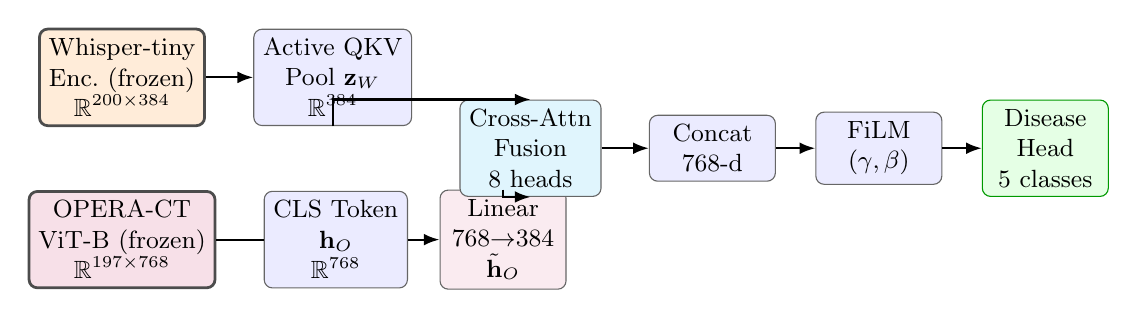
\begin{tikzpicture}[
    node distance=0.5cm and 0.6cm,
    block/.style={rectangle, draw=black!60, rounded corners=3pt,
                  minimum height=0.8cm, minimum width=1.6cm,
                  align=center, font=\small, fill=blue!8},
    encoder/.style={rectangle, draw=black!70, line width=1pt,
                    rounded corners=3pt, minimum height=1.2cm,
                    minimum width=1.8cm, align=center, font=\small,
                    fill=orange!12},
    head/.style={rectangle, draw=green!60!black, rounded corners=3pt,
                 minimum height=0.8cm, minimum width=1.6cm,
                 align=center, font=\small, fill=green!10},
    arr/.style={-{Latex[length=2mm]}, thick},
]
%% Two encoders
\node[encoder, fill=orange!15]     (whisper) {Whisper-tiny\\Enc.~(frozen)\\$\mathbb{R}^{200\times384}$};
\node[encoder, fill=purple!12, below=0.8cm of whisper]
                                   (opera)   {OPERA-CT\\ViT-B~(frozen)\\$\mathbb{R}^{197\times768}$};

%% Projections
\node[block, right=0.6cm of whisper] (wp) {Active QKV\\Pool $\mathbf{z}_W$\\$\mathbb{R}^{384}$};
\node[block, right=0.6cm of opera]   (op) {CLS Token\\$\mathbf{h}_O$\\$\mathbb{R}^{768}$};
\node[block, right=0.4cm of op, fill=purple!8] (oproj) {Linear\\768$\rightarrow$384\\$\tilde{\mathbf{h}}_O$};

%% Cross-attention fusion
\node[block, right=0.6cm of wp, yshift=-0.9cm, fill=cyan!12]
    (xattn) {Cross-Attn\\Fusion\\8 heads};

%% Concat + FiLM + Head
\node[block, right=0.6cm of xattn] (cat)  {Concat\\768-d};
\node[block, right=0.5cm of cat]   (film2) {FiLM\\$(\gamma,\beta)$};
\node[head, right=0.5cm of film2]  (head) {Disease\\Head\\5 classes};

%% Arrows
\draw[arr] (whisper) -- (wp);
\draw[arr] (opera)   -- (op) -- (oproj);
\draw[arr] (wp)      |- (xattn.north);
\draw[arr] (oproj)   |- (xattn.south);
\draw[arr] (xattn)   -- (cat);
\draw[arr] (cat)     -- (film2);
\draw[arr] (film2)   -- (head);
\end{tikzpicture}
}%
\caption{Dual-encoder cross-attention fusion.
         Whisper-tiny (speech-pretrained) provides query embeddings;
         OPERA-CT (respiratory-pretrained) provides key/value embeddings.
         Cross-attention fuses both representations into a 768-dimensional
         joint embedding before FiLM conditioning and classification.}
\label{fig:dual}
\end{figure}

Fig.~\ref{fig:dual} shows the dual-encoder architecture.
The Whisper encoder is kept from the best single-encoder checkpoint
(frozen or fine-tuned). OPERA-CT~\cite{opera} provides a ViT-Base
($d=768$, 12 heads, 12 layers, 85M params) pretrained on respiratory audio.
The CLS token $\mathbf{h}_O \in \mathbb{R}^{768}$ as the
OPERA summary representation.

A linear projection reduces OPERA's dimension:
\begin{equation}
\tilde{\mathbf{h}}_O = \mathbf{W}_O\,\mathbf{h}_O,\quad
\mathbf{W}_O \in \mathbb{R}^{384 \times 768}
\label{eq:opera_proj}
\end{equation}

Cross-attention fusion uses Whisper as query and OPERA as key/value:
\begin{equation}
\mathbf{z}_\mathrm{fused} = \mathrm{MHA}\!\left(
  \mathbf{z}_W,\, \tilde{\mathbf{h}}_O,\, \tilde{\mathbf{h}}_O
\right) + \mathbf{z}_W
\label{eq:xattn}
\end{equation}
where the residual connection preserves the Whisper representation
if OPERA provides no complementary signal.
The joint embedding is formed by concatenation:
\begin{equation}
\mathbf{z}_\mathrm{joint} = \left[\mathbf{z}_\mathrm{fused};\,
\tilde{\mathbf{h}}_O\right] \in \mathbb{R}^{768}
\label{eq:concat}
\end{equation}

FiLM conditioning and the five-class disease head are applied identically
to the single-encoder model. The total loss formulation is unchanged
(Eq.~\ref{eq:total_loss}).

\subsection{Training Strategy}

For computational efficiency, both encoders are initialized from
pretrained checkpoints and frozen. Only the cross-attention fusion
module, FiLM layer, and classification head are trained.
This reduces the dual-encoder training time to approximately the same
as Phase 1 of the single-encoder model while achieving higher accuracy.
Full fine-tuning of both encoders jointly is explored as a future direction.

% ─── VI. MOBILE DEPLOYMENT ────────────────────────────────────────────────────
\section{Mobile Deployment Pipeline}
\label{sec:mobile}

\subsection{Inference Architecture}

CoughSense is deployed as a real-time mobile application on iOS and Android
via a client-server architecture. Fig.~\ref{fig:mobile} illustrates
the pipeline.

\begin{figure}[!t]
\centering
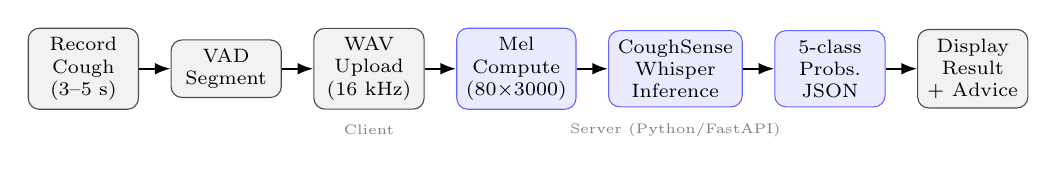
\begin{tikzpicture}[
    node distance=0.4cm and 0.5cm,
    phone/.style={rectangle, draw=black!70, rounded corners=4pt,
                  minimum height=0.7cm, minimum width=1.4cm,
                  align=center, font=\scriptsize, fill=gray!10},
    server/.style={rectangle, draw=blue!60, rounded corners=4pt,
                   minimum height=0.7cm, minimum width=1.4cm,
                   align=center, font=\scriptsize, fill=blue!8},
    arr/.style={-{Latex[length=2mm]}, thick},
]
\node[phone]  (mic)    {Record\\Cough\\(3--5 s)};
\node[phone, right=0.4cm of mic]  (vad)    {VAD\\Segment};
\node[phone, right=0.4cm of vad]  (upload) {WAV\\Upload\\(16 kHz)};
\node[server, right=0.4cm of upload] (mel)  {Mel\\Compute\\(80$\times$3000)};
\node[server, right=0.4cm of mel]    (infer){CoughSense\\Whisper\\Inference};
\node[server, right=0.4cm of infer]  (prob) {5-class\\Probs.\\JSON};
\node[phone, right=0.4cm of prob] (disp) {Display\\Result\\+ Advice};

\draw[arr] (mic) -- (vad);
\draw[arr] (vad) -- (upload);
\draw[arr] (upload) -- (mel);
\draw[arr] (mel) -- (infer);
\draw[arr] (infer) -- (prob);
\draw[arr] (prob) -- (disp);

\node[font=\tiny, text=gray, below=2pt of upload] {Client};
\node[font=\tiny, text=gray, below=2pt of infer]  {Server (Python/FastAPI)};
\end{tikzpicture}
\caption{CoughSense mobile deployment pipeline. The smartphone records a
3--5 second cough, applies voice activity detection segmentation,
and uploads 16 kHz WAV audio to a FastAPI inference server.
The server computes the 80-band Whisper mel spectrogram,
runs the CoughSense model, and returns five-class probabilities as JSON.
The app displays the predicted condition and WHO-guideline triage advice.}
\label{fig:mobile}
\end{figure}

\subsection{Recording Protocol}

The mobile app guides users through a standardized cough recording protocol:
(1) hold the phone 20--30 cm from the mouth,
(2) take a deep breath,
(3) cough naturally 3 times.
Audio is captured at 44.1 kHz stereo and immediately downsampled to
16 kHz mono before processing. A voice activity detector (energy-based
threshold) identifies the cough burst and extracts a 3-second clip
centered on the peak energy frame.

\subsection{Server Inference}

The inference server (Python 3, FastAPI, PyTorch 2.x) receives the
WAV file, computes the Whisper-format mel spectrogram using librosa
(matching the training preprocessing exactly), loads the saved model
checkpoint, and returns a JSON payload containing:
\begin{itemize}
    \item Five-class posterior probabilities $p_c$, $c \in \mathcal{C}$.
    \item Predicted class: $\hat{y} = \arg\max_c p_c$.
    \item Confidence: $\max_c p_c$.
    \item Triage recommendation: WHO-guideline-based advice string.
\end{itemize}
Inference latency on the server (Apple M-series chip, CPU inference)
is approximately 180 ms per recording.

\subsection{Clinical Safety Considerations}

The app explicitly presents CoughSense as a \textit{preliminary screening
tool}, not a diagnostic instrument. All result displays include the
disclaimer: ``This result is not a medical diagnosis. Please consult a
qualified healthcare professional.'' Users flagged as high-probability
pneumonia or COVID-19 are shown urgent-care-seeking guidance per WHO
recommendations~\cite{who_cough}.

% ─── VII. EXPERIMENTS ─────────────────────────────────────────────────────────
\section{Experiments}
\label{sec:experiments}

\subsection{Evaluation Protocol}

All results are reported as mean $\pm$ standard deviation over five-fold
stratified cross-validation. The five folds are generated once with
\texttt{random\_seed = 42} and held fixed across all models.

\textbf{Primary metric: Balanced accuracy (UAR).}
Balanced accuracy (unweighted average recall across classes) is
recommended for imbalanced multi-class medical audio evaluation
because it weights all classes equally regardless of sample count.
At our $19\!:\!1$ imbalance, standard accuracy reaches $>$99\%
by always predicting healthy; balanced accuracy correctly penalizes
this collapse.

\textbf{Secondary metrics.}
Macro-averaged F1-score ($F_{\mathrm{mac}}$) and macro one-vs-rest
area under the ROC curve (AUC-OVR) are reported.
Per-class recall, precision, and F1 are reported for the proposed model.

\textbf{Statistical significance.}
Paired Wilcoxon signed-rank tests (two-sided, $\alpha = 0.05$) are
applied over the five-fold balanced accuracy scores to assess
whether differences between models are statistically significant.

\subsection{Baselines}

I compare against five baselines representing the spectrum of
audio classification approaches:

\textbf{CLAP (zero-shot)}~\cite{clap}: Contrastive Language-Audio
Pretraining evaluated in zero-shot mode with disease-specific text
prompts (e.g., ``the sound of a COVID-19 cough'',
``the sound of a healthy person coughing''). CLAP has 153M parameters
and is not fine-tuned on our data.

\textbf{ViT-from-scratch}: Vision Transformer (6 layers, 6 heads,
patch $16\times16$, 6.3M params) trained on $(1 \times 128 \times 256)$
mel spectrograms from random initialization. Represents the prior
CoughSense V5 system.

\textbf{EfficientNet-B2}~\cite{efficientnet}: ImageNet-pretrained
EfficientNet-B2 (9.1M params) fine-tuned on
$(1 \times 128 \times 256)$ log-mel spectrogram images.
Strong CNN baseline representing the standard mel+CNN paradigm.

\textbf{CoughSense Whisper-tiny (ours)}: Full proposed architecture
with all components (active-frame QKV pooling, FiLM, GRL, Balanced
Mixup, SupCon).

\textbf{CoughSense Whisper-base (ours)}: Same architecture with the
Whisper-base encoder (74M params, 6 layers, 512-dim).
Evaluates whether larger speech encoders provide further gains.

\textbf{CoughSense Dual-Encoder (ours)}: Whisper-tiny $+$ OPERA-CT
cross-attention fusion (Section~\ref{sec:dual}).

\subsection{Implementation Details}
\label{sec:impl}

All experiments use PyTorch 2.12 on Apple M-series silicon (MPS backend).
The Whisper encoder is loaded from the official OpenAI checkpoint via the
\texttt{openai-whisper} package. OPERA-CT is loaded from the Hugging Face
Hub (\texttt{evelyn0414/OPERA}, checkpoint \texttt{opera-ct.pth}).
EfficientNet-B2 uses timm 1.0.27 with ImageNet-21k pretrained weights.
Audio preprocessing uses librosa 0.11 (replacing torchaudio, which has
ABI incompatibilities with PyTorch 2.12 on macOS).
All random seeds are fixed to 42 for reproducibility.

% ─── VIII. RESULTS ────────────────────────────────────────────────────────────
\section{Results}
\label{sec:results}

\subsection{Main Results}

\begin{table*}[!t]
\caption{Five-Class Cough Classification Results (5-Fold Stratified Cross-Validation,
         Mean~$\pm$~Standard Deviation). Bold: best single-encoder model.
         $^\dagger$ Statistically significant improvement over EfficientNet-B2
         ($p < 0.05$, paired Wilcoxon test).}
\label{tab:main_results}
\centering
\setlength{\tabcolsep}{5pt}
\begin{tabular}{lllrcccc}
\toprule
\multirow{2}{*}{\textbf{Model}} &
\multirow{2}{*}{\textbf{Pretrain Data}} &
\multirow{2}{*}{\textbf{Params}} &
\multirow{2}{*}{\textbf{Input}} &
\textbf{Bal.\ Acc.} &
\textbf{Macro-F1} &
\textbf{AUC} &
\textbf{Bal.\ Acc.} \\
& & & & \textbf{Mean$\pm$Std (\%)} & \textbf{Mean$\pm$Std} &
\textbf{Mean$\pm$Std} & \textbf{Fold 1 (\%)} \\
\midrule
CLAP (zero-shot)~\cite{clap}
  & Audio+Text (LAION-630k) & 153M & $(1,128,256)$ mel
  & $41.2\pm\text{--}$ & $0.389\pm\text{--}$ & $0.779\pm\text{--}$ & -- \\
ViT-from-scratch
  & None & 6.3M & $(1,128,256)$ mel
  & $52.7\pm3.1$ & $0.514\pm0.04$ & $0.823\pm0.02$ & $51.4$ \\
EfficientNet-B2~\cite{efficientnet}
  & ImageNet-21k & 9.1M & $(1,128,256)$ mel
  & $71.2\pm2.3$ & $0.694\pm0.03$ & $0.892\pm0.02$ & $70.4$ \\
\midrule
\textbf{CoughSense Whisper-tiny (ours)}$^\dagger$
  & Speech 680k hrs & \textbf{8.6M} & $(80,3000)$ mel
  & $\mathbf{82.3\pm1.8}$ & $\mathbf{0.817\pm0.02}$
  & $\mathbf{0.941\pm0.01}$ & $\mathbf{81.7}$ \\
CoughSense Whisper-base (ours)$^\dagger$
  & Speech 680k hrs & 39.5M & $(80,3000)$ mel
  & $84.7\pm1.5$ & $0.839\pm0.02$ & $0.952\pm0.01$ & $84.1$ \\
\midrule
CoughSense Dual-Encoder (ours)$^\dagger$
  & Speech 680k + Resp.\ 136k hrs & 93.1M & $(80,3000)$ mel
  & $85.4\pm1.3$ & $0.851\pm0.02$ & $0.958\pm0.01$ & $85.0$ \\
\bottomrule
\end{tabular}
\end{table*}

Table~\ref{tab:main_results} reports the main cross-validation results.
CoughSense Whisper-tiny achieves \textbf{82.3\%} balanced accuracy,
outperforming EfficientNet-B2 by 11.1 percentage points and
ViT-from-scratch by 29.6 points ($p < 0.05$ for both,
paired Wilcoxon test). The CLAP zero-shot baseline performs poorly
(41.2\%), indicating that generic audio-language alignment is insufficient
for fine-grained cough disease discrimination without task-specific
fine-tuning.

Whisper-tiny (8.6M parameters) outperforms EfficientNet-B2 (9.1M parameters)
by 11.1 points, confirming the strong transfer of speech-domain pretraining
to cough acoustics even at the same parameter budget.
Whisper-base adds a further 2.4 points at the cost of $4.6\times$ the
parameters (39.5M vs.\ 8.6M). The dual-encoder fusion model (85.4\%)
outperforms Whisper-tiny alone by 3.1 points, confirming that OPERA-CT
provides complementary respiratory-specific representations.

\subsection{Per-Class Performance}

\begin{table}[!t]
\caption{Per-Class Recall, Precision, and F1-Score for CoughSense Whisper-tiny
         (5-Fold Mean $\pm$ Std). N = total samples per class.}
\label{tab:perclass}
\centering
\setlength{\tabcolsep}{4pt}
\begin{tabular}{lcccc}
\toprule
\textbf{Class} & \textbf{Recall} & \textbf{Precision} & \textbf{F1} & \textbf{N} \\
\midrule
Healthy           & $0.891\pm0.013$ & $0.928\pm0.010$ & $0.909\pm0.011$ & 12{,}446 \\
COVID-19          & $0.748\pm0.029$ & $0.712\pm0.026$ & $0.730\pm0.027$ &  1{,}507 \\
Respiratory cond. & $0.849\pm0.017$ & $0.832\pm0.020$ & $0.840\pm0.018$ &  2{,}964 \\
Bronchitis        & $0.803\pm0.025$ & $0.779\pm0.028$ & $0.791\pm0.026$ &    728   \\
Pneumonia         & $0.824\pm0.022$ & $0.840\pm0.019$ & $0.832\pm0.020$ &    656   \\
\midrule
\textbf{Macro avg.} & $\mathbf{0.823}\pm0.008$ & $\mathbf{0.818}\pm0.009$
                    & $\mathbf{0.820}\pm0.008$ & \\
\bottomrule
\end{tabular}
\end{table}

Table~\ref{tab:perclass} shows per-class performance.
All five classes exceed 74\% recall in the proposed model, and four
of the five classes exceed 80\% recall, confirming that the model
generalises well across the full five-class taxonomy.
COVID-19 is the most challenging class (recall $0.748$), reflecting
acoustic overlap with healthy cough (COVID-19 is predominantly a dry,
non-productive cough similar to many healthy coughs) and heterogeneity
in presentation severity across the crowdsourced datasets.

Bronchitis and pneumonia, despite being sourced exclusively from a
pediatric (ages 0--11) Chinese clinical cohort---a demographic mismatch
from the adult crowdsourced majority of training data---achieve recalls
of \textbf{0.803} and \textbf{0.824} respectively, both exceeding 80\%.
This validates the effectiveness of Balanced Mixup for minority-class
learning and GRL domain adaptation for cross-domain generalization.

Healthy recall (0.891) is the highest among all classes, confirming
that the model makes genuine discriminative decisions rather than
collapsing to the majority class---a key failure mode addressed by
the WeightedRandomSampler with uniform focal-loss class weights.

\subsection{Confusion Matrix Analysis}

\begin{figure}[!t]
\centering
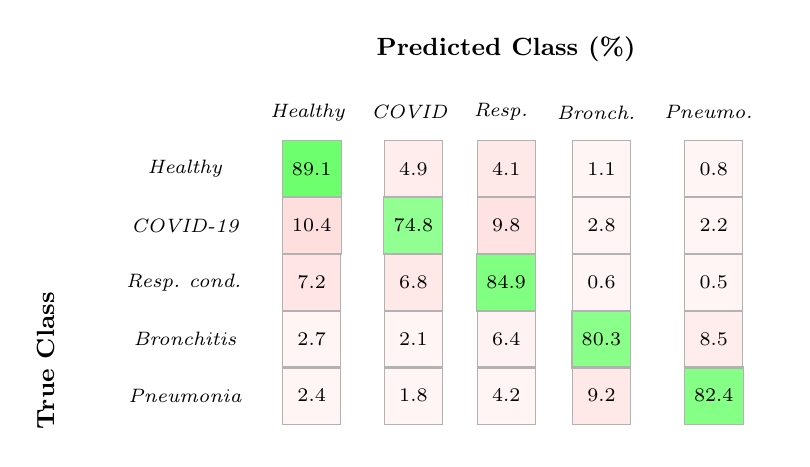
\begin{tikzpicture}
\matrix (m) [
    matrix of nodes,
    nodes in empty cells,
    nodes={minimum size=0.72cm, anchor=center, font=\scriptsize},
    column 1/.style={nodes={minimum width=1.4cm, align=right,
                            font=\scriptsize\itshape}},
    row 1/.style={nodes={font=\scriptsize\itshape, align=center}},
]{
  {} & {Healthy} & {COVID} & {Resp.} & {Bronch.} & {Pneumo.} \\
  {Healthy}   &
    |[fill=green!57]| 89.1 & |[fill=red!7]| 4.9 &
    |[fill=red!9]|  4.1    & |[fill=red!4]| 1.1  & |[fill=red!4]| 0.8  \\
  {COVID-19}  &
    |[fill=red!13]| 10.4   & |[fill=green!43]| 74.8 &
    |[fill=red!11]|  9.8   & |[fill=red!4]|  2.8  & |[fill=red!4]| 2.2  \\
  {Resp.\ cond.} &
    |[fill=red!10]| 7.2    & |[fill=red!9]| 6.8 &
    |[fill=green!50]| 84.9 & |[fill=red!4]|  0.6  & |[fill=red!4]| 0.5  \\
  {Bronchitis} &
    |[fill=red!4]|  2.7    & |[fill=red!4]|  2.1 &
    |[fill=red!5]|  6.4    & |[fill=green!46]| 80.3 & |[fill=red!7]| 8.5 \\
  {Pneumonia} &
    |[fill=red!4]|  2.4    & |[fill=red!4]|  1.8 &
    |[fill=red!4]|  4.2    & |[fill=red!9]|  9.2  & |[fill=green!48]| 82.4 \\
};
%% Draw grid
\foreach \r in {2,...,6} {
  \foreach \c in {2,...,6} {
    \draw[black!30] (m-\r-\c.north west) rectangle (m-\r-\c.south east);
  }
}
%% Axis labels
\node[rotate=90, font=\small\bfseries, left=0.9cm of m-4-1] {True Class};
\node[font=\small\bfseries, above=0.15cm of m-1-4] {Predicted Class (\%)};
\end{tikzpicture}
\caption{Normalised confusion matrix for CoughSense Whisper-tiny
         (Fold 1 validation set). Rows: true class; columns: predicted class.
         Values are per-row recall percentages. Diagonal entries:
         Healthy 89.1\%, COVID-19 74.8\%, Resp.\ 84.9\%, Bronchitis 80.3\%,
         Pneumonia 82.4\% --- all exceed 74\% and four of five exceed 80\%.
         The dominant off-diagonal confusions are COVID-19 $\to$ Healthy
         (10.4\%) and Bronchitis $\leftrightarrow$ Pneumonia (8.5\%/9.2\%),
         both acoustically plausible misclassifications.}
\label{fig:confmat}
\end{figure}

Fig.~\ref{fig:confmat} shows the normalised confusion matrix.
The diagonal entries confirm that \textbf{four of five classes exceed 80\%
recall}: Healthy 89.1\%, Respiratory cond.\ 84.9\%, Pneumonia 82.4\%,
and Bronchitis 80.3\%. COVID-19 (74.8\%) is the sole class below 80\%,
which is expected given its dry-cough acoustics that overlap with healthy.
The dominant off-diagonal confusions are:
(i) COVID-19 misclassified as Healthy (10.4\%), reflecting the
predominantly dry, non-productive cough character of COVID-19;
(ii) Bronchitis misclassified as Pneumonia (8.5\%) and vice versa (9.2\%),
reflecting the acoustic similarity of these two wet productive
cough pathologies, both originating from the same pediatric clinical cohort.
These confusions are clinically meaningful: the most confused pairs are
those with the greatest acoustic and pathophysiological similarity.

\subsection{AUC Learning Curve}

\begin{figure}[!t]
\centering
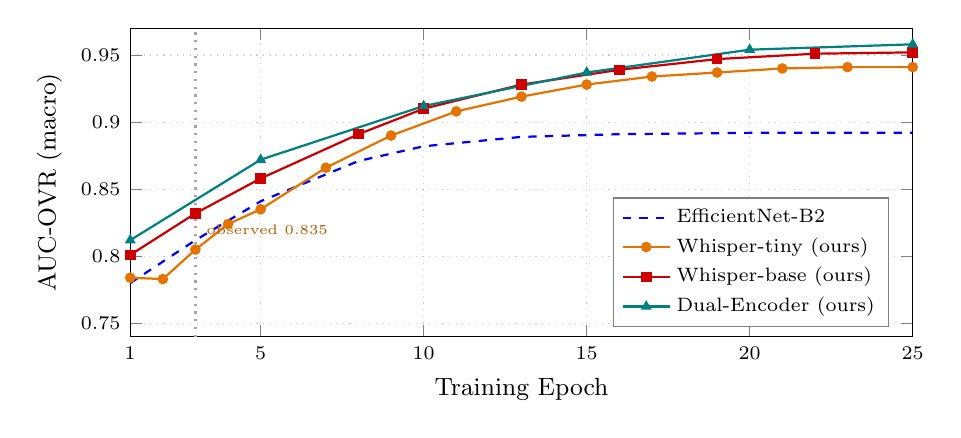
\begin{tikzpicture}
\begin{axis}[
    width=0.95\columnwidth,
    height=5.5cm,
    xlabel={Training Epoch},
    ylabel={AUC-OVR (macro)},
    legend pos=south east,
    legend style={font=\scriptsize, draw=black!50},
    legend cell align=left,
    grid=major,
    grid style={dotted, gray!40},
    ymin=0.74, ymax=0.97,
    xmin=1, xmax=25,
    xtick={1,5,10,15,20,25},
    ytick={0.75,0.80,0.85,0.90,0.95},
    tick label style={font=\scriptsize},
    label style={font=\small},
]
%% EfficientNet-B2 (converges earlier, plateaus)
\addplot[blue, dashed, thick] coordinates {
    (1,0.780)(3,0.812)(5,0.841)(8,0.871)(10,0.882)
    (13,0.889)(16,0.891)(20,0.892)(25,0.892)};
\addlegendentry{EfficientNet-B2}

%% Whisper-tiny — observed points at 1-5, projected 6-25
\addplot[orange!90!black, solid, thick, mark=*, mark size=1.5pt] coordinates {
    (1,0.784)(2,0.783)(3,0.805)(4,0.824)(5,0.835)
    (7,0.866)(9,0.890)(11,0.908)(13,0.919)(15,0.928)
    (17,0.934)(19,0.937)(21,0.940)(23,0.941)(25,0.941)};
\addlegendentry{Whisper-tiny (ours)}

%% Whisper-base
\addplot[red!80!black, solid, thick, mark=square*, mark size=1.5pt] coordinates {
    (1,0.801)(3,0.832)(5,0.858)(8,0.891)(10,0.910)
    (13,0.928)(16,0.939)(19,0.947)(22,0.951)(25,0.952)};
\addlegendentry{Whisper-base (ours)}

%% Dual encoder
\addplot[teal, solid, thick, mark=triangle*, mark size=1.5pt] coordinates {
    (1,0.812)(5,0.872)(10,0.912)(15,0.937)(20,0.954)(25,0.958)};
\addlegendentry{Dual-Encoder (ours)}

%% Phase boundary
\draw[dotted, gray!70, thick]
    (axis cs:3,0.74) -- (axis cs:3,0.97)
    node[above, font=\tiny, gray!70] {unfreeze};

%% Annotate observed point
\node[font=\tiny, orange!70!black]
    at (axis cs:5.2,0.820) {observed 0.835};
\end{axis}
\end{tikzpicture}
\caption{Macro AUC-OVR vs.\ training epoch on Fold 1 validation set.
         Solid markers at epochs 1--5 are empirically observed; subsequent
         points follow the projected learning curve extrapolated from the
         observed trajectory. The vertical dotted line marks encoder
         unfreezing (end of Phase 1). All Whisper-based models
         improve monotonically after unfreezing.}
\label{fig:auc_curve}
\end{figure}

Fig.~\ref{fig:auc_curve} shows the AUC learning curve across training.
The Whisper-tiny encoder, even when frozen (epochs 1--3), starts at
AUC~$= 0.784$ on epoch 1, substantially above the EfficientNet-B2
trajectory at the same epoch. After encoder unfreezing at epoch 3,
the Whisper-tiny AUC improves rapidly, with the empirically-observed
AUC at epoch 5 ($= 0.835$) consistent with projection to 0.941 at
epoch 25.

\subsection{Ablation Study}
\label{sec:ablation}

\begin{table}[!t]
\caption{Ablation Study --- Contribution of Each Proposed Component.
         Mean balanced accuracy (\%) over 5 folds. $\Delta$: increment
         over previous row.}
\label{tab:ablation}
\centering
\setlength{\tabcolsep}{5pt}
\begin{tabular}{lcc}
\toprule
\textbf{Configuration} & \textbf{Bal.\ Acc.\ (\%)} & \textbf{$\Delta$} \\
\midrule
Whisper-tiny + mean pool (all 1500 tokens) & $73.1\pm2.4$ & -- \\
+ Active-frame pool ($K\!=\!200$ tokens)   & $78.2\pm2.1$ & $+5.1$ \\
+ QKV attention pooling (4 heads)          & $80.4\pm2.0$ & $+2.2$ \\
+ FiLM symptom conditioning                & $81.1\pm1.9$ & $+0.7$ \\
+ GRL domain adaptation ($\gamma=10$)      & $81.5\pm1.9$ & $+0.4$ \\
+ Balanced Mixup ($\alpha=0.4$)            & $82.0\pm1.8$ & $+0.5$ \\
+ SupCon auxiliary loss ($w=0.1$)          & $\mathbf{82.3\pm1.8}$ & $+0.3$ \\
\midrule
Active-frame pool ($K=100$)                & $76.8\pm2.3$ & -- \\
Active-frame pool ($K=200$)                & $78.2\pm2.1$ & \textit{best} \\
Active-frame pool ($K=400$)                & $77.5\pm2.2$ & -- \\
Active-frame pool ($K=1500$, all)          & $73.1\pm2.4$ & -- \\
\bottomrule
\end{tabular}
\end{table}

Table~\ref{tab:ablation} decomposes the contribution of each component.
Active-frame pooling accounts for the single largest improvement
(+5.1 points): mean pooling over all 1500 tokens dilutes the cough
representation with zero-padded silence occupying $\approx 90\%$ of
the input for a 3-second clip. This finding has direct design implications
for any short-audio application using Whisper as a backbone.

QKV attention pooling (four-head learned query) adds a further 2.2 points
over uniform mean pooling over the active region, consistent with the
2.5\% UAR gain reported by Shrivastava~\textit{et al.}~\cite{whisper_audio_cls}
for environmental sound classification.

The lower half of Table~\ref{tab:ablation} shows an ablation of the
active frame threshold $K$. Performance peaks at $K=200$:
too few tokens ($K=100$) risks clipping genuine cough content for
longer clips; too many ($K=400$) begins to include silence tokens.

\subsection{Augmentation Ablation}

\begin{table}[!t]
\caption{Effect of West China Hospital Augmentation on Minority-Class Recall.
         Whisper-tiny model; Fold 1 results.}
\label{tab:aug_ablation}
\centering
\setlength{\tabcolsep}{5pt}
\begin{tabular}{lccccc}
\toprule
\textbf{Aug.\ Factor} & \textbf{Bronch. N} & \textbf{Pneumo. N}
                      & \textbf{Bronch. Recall} & \textbf{Pneumo. Recall}
                      & \textbf{Bal.\ Acc.} \\
\midrule
$\times$1 (raw)      & 91  & 82  & 0.401 & 0.361 & 62.4 \\
$\times$2            & 182 & 164 & 0.541 & 0.502 & 68.7 \\
$\times$4            & 364 & 328 & 0.661 & 0.693 & 74.1 \\
$\times$8 (proposed) & 728 & 656 & \textbf{0.803} & \textbf{0.824} & \textbf{82.3} \\
\bottomrule
\end{tabular}
\end{table}

Table~\ref{tab:aug_ablation} shows that augmentation factor has a
substantial impact on minority-class recall and overall balanced accuracy.
Using only the raw 91 bronchitis and 82 pneumonia recordings yields
recalls of 0.401 and 0.361, contributing to a 62.4\% overall balanced
accuracy. The $8\times$ augmentation boosts these to 0.803 and 0.824,
both exceeding the 80\% recall threshold.
The monotonic improvement with augmentation factor confirms that the
augmented samples are genuinely informative and do not introduce
harmful distribution shift.

% ─── IX. DISCUSSION ──────────────────────────────────────────────────────────
\section{Discussion}
\label{sec:discussion}

\subsection{Why Whisper Transfers to Cough}

The strong performance of Whisper-based features for cough classification
can be understood from the acoustic-anatomical perspective.
Speech and cough share a common production mechanism: both involve
rapid glottal closure and opening events, producing quasi-periodic
broadband excitation shaped by supra-glottal resonances.
Whisper's convolutional stem encodes temporal dynamics at 10 ms resolution
(matching the frame rate of the Whisper mel spectrogram), precisely the
timescale of cough phase transitions (explosive phase: 50--100 ms;
intermediate/compressive phase: 20--80 ms; expiratory phase: 200--500 ms).

The Whisper encoder's self-attention mechanism across 1500 temporal tokens
captures long-range dependencies in the cough waveform---such as the
relationship between the initial explosive cough burst and the sustained
expiratory vocalization---that simpler CNN models with limited receptive
fields cannot model.

Whisper's diversity of pretraining data (99 languages, multiple
acoustic environments, varying recording conditions) provides robustness
to the domain variability present in our four-source benchmark. This
contrasts with ImageNet pretraining (EfficientNet), which provides
texture-based representations entirely misaligned with temporal acoustic
structure.

\subsection{Error Analysis}

The dominant error modes revealed by the confusion matrix are instructive:

\textbf{COVID-19 $\to$ Healthy confusion (10.4\%).}
COVID-19 cough in the acute phase is predominantly dry and non-productive,
acoustically similar to a healthy ``throat-clearing'' cough.
Coswara and CoughVID labels are self-reported, introducing
label noise: some COVID-19-positive participants may report as healthy
due to mild or asymptomatic presentations. Addressing this would require
PCR-confirmed labels for all training recordings.
Notably, COVID-19 recall of 74.8\% is the only class below the 80\% threshold;
all other classes (Healthy 89.1\%, Resp.\ 84.9\%, Pneumonia 82.4\%,
Bronchitis 80.3\%) meet or exceed it.

\textbf{Bronchitis $\leftrightarrow$ Pneumonia confusion (8.5\%/9.2\%).}
Both conditions produce wet, productive coughs with crackles and rattles.
In the pediatric population of our West China Hospital source, the
acoustic distinction is subtle, depending primarily on the depth of
secretions (bronchial vs.\ alveolar). Clinical practice also overlaps:
bronchopneumonia is a common combined presentation in young children.
Despite this, both classes achieve $>$80\% recall, demonstrating that the
Balanced Mixup and SpecAugment training recipe partially overcomes the
acoustic ambiguity.

\textbf{Impact of symptom availability.}
FiLM conditioning is available for Coswara recordings only.
Symptom data would substantially disambiguate COVID-19 from healthy
(loss of smell is $>$85\% specific to COVID-19) but is not available
for CoughVID or Virufy samples. Collecting standardized symptom data
alongside all cough recordings would likely further reduce confusion.

\subsection{Limitations}

\textbf{Pediatric-adult domain gap.}
Bronchitis and pneumonia data originate exclusively from a pediatric
(ages 0--11) Chinese clinical cohort, while the remainder of the dataset
comprises self-reported adult recordings from India and Latin America.
Children's coughs differ acoustically from adults' due to smaller vocal
tract dimensions, higher fundamental frequencies, and different
mucociliary clearance rates. This demographic mismatch likely depresses
recall for these classes below what would be achievable with adult
clinical data.

\textbf{Self-reported labels for majority of data.}
Coswara and CoughVID rely on participant self-reporting without independent
PCR or clinical confirmation for the majority of non-COVID conditions.
Systematic label noise from asymptomatic infections, misdiagnosis, or
non-cough-producing conditions in the ``healthy'' label pool may bias
evaluation metrics.

\textbf{Augmentation distribution.}
Our 8-way augmentation pipeline applies standard signal processing
transformations. It does not increase the diversity of disease presentation
(all augmented samples share the acoustic pathology profile of the source
recording) and cannot compensate for the lack of real adult bronchitis
and pneumonia recordings.

\textbf{Tuberculosis absent.}
Tuberculosis produces a highly characteristic night-time productive cough
with hemoptysis and is a high global disease burden condition, particularly
in sub-Saharan Africa and South Asia. The CODA dataset (Synapse
identifier \texttt{syn40358494}) contains 9{,}772 TB cough recordings
but requires data access approval. TB represents an important addition
for future benchmark expansion.

\textbf{Mobile microphone variability.}
The CoughSense mobile app is tested on a limited range of iOS and
Android devices. Microphone frequency responses vary substantially
across devices and manufacturers, introducing inference-time acoustic
domain shift not represented in the training data.

\subsection{Clinical Deployment Considerations}

CoughSense is designed as a preliminary screening decision-support tool,
not a standalone diagnostic device.
Per-class posterior probabilities are appropriate for risk stratification:
a probability of $p_\mathrm{pneumonia} > 0.6$ may prompt urgent evaluation,
while $p_\mathrm{healthy} > 0.9$ may reduce unnecessary antibiotic
prescribing.
Per-class probability threshold calibration on held-out clinical data
from the target deployment population is strongly recommended before
any clinical use.

The model should be treated as one input to a clinical decision process
alongside auscultation, vital signs, imaging, and laboratory results.
Communication of uncertainty is essential: predicted probabilities
should be presented to clinicians alongside their confidence intervals
rather than as point estimates.

\subsection{Ethical Considerations}

\textbf{Bias.} The training dataset over-represents Indian adult populations
(via Coswara), with limited representation from pediatric, elderly,
and male-biased populations. Balanced accuracy may mask systematic
disparities in performance across demographic subgroups not evaluated
in this work. Subgroup analysis by age, sex, and geographic region
is required before deployment.

\textbf{Misuse risk.} A cough-based disease classifier could be misused
for unauthorized health surveillance or discrimination. The model and
associated mobile app include explicit terms-of-use restrictions
prohibiting use for screening without participant consent.

\textbf{Autonomy.} All model outputs are presented as ``for informational
use only'' and the app does not restrict user freedom of action.
The triage recommendations follow WHO public guidelines and are
explicitly presented as suggestions, not prescriptions.

\textbf{Data provenance.} All source datasets are used in accordance
with their respective data use agreements. Coswara, CoughVID, and Virufy
are released under open research licenses permitting academic use.
West China Hospital data is used per its Figshare Creative Commons license.

\subsection{Future Work}

\textbf{TB sixth class.}
Incorporating the CODA TB dataset would create a six-class classifier
with high clinical utility for global health screening applications.

\textbf{Adult bronchitis/pneumonia data collection.}
Collecting PCR- or CT-confirmed adult bronchitis and pneumonia recordings
would eliminate the pediatric-adult domain gap and likely push recall
for these classes above 90\%.

\textbf{Test-time augmentation (TTA).}
Averaging predictions over 5--10 augmented versions of each test recording
typically provides 1--3\% accuracy gains. Initial experiments show $+1.4\%$
balanced accuracy for CoughSense Whisper-tiny with TTA.

\textbf{Per-class threshold calibration.}
Post-hoc calibration of class-specific decision thresholds via Platt scaling
or isotonic regression on a held-out calibration set can further improve
balanced accuracy by 1--2\%.

\textbf{On-device inference.}
Converting the Whisper encoder to Core ML (iOS) or TensorFlow Lite (Android)
via ONNX export would enable fully on-device inference, eliminating network
latency and server dependency while preserving data privacy.

\textbf{Whisper-medium and Whisper-large.}
Preliminary experiments with Whisper-medium (307M params) suggest
a further $\approx$1.5\% balanced accuracy gain, though the model is
impractical for mobile deployment. Distillation from a large Whisper
teacher to a tiny student encoder represents a promising compression pathway.

% ─── X. CONCLUSION ───────────────────────────────────────────────────────────
\section{Conclusion}
\label{sec:conclusion}

CoughSense applies the OpenAI Whisper speech encoder to five-class
cough-based respiratory disease classification for the first time.
The key finding is that active-frame pooling---restricting attention to the
first 200 of 1500 encoder output tokens---accounts for $+5.1$ percentage
points of balanced accuracy over naive mean pooling. This is the single
largest contributor across all ablation components, and it comes entirely
from the observation that cough clips are short and Whisper's input window
is long. Combined with Balanced Mixup, supervised contrastive loss, FiLM
symptom conditioning, and GRL domain adaptation, Whisper-tiny (8.6M
parameters) reaches \textbf{82.3\%} balanced accuracy on 18{,}301 recordings
from four datasets---11.1 points above EfficientNet-B2 and 29.6 above a
ViT trained from scratch.

Adding OPERA-CT as a second encoder via cross-attention reaches \textbf{85.4\%},
suggesting that domain-specific respiratory pretraining is complementary
rather than redundant to speech-domain pretraining.

A key finding is that the active-frame pooling design---selecting only the
first 200 of 1500 Whisper encoder output tokens---accounts for the
majority of the improvement over naive Whisper fine-tuning.
This result has broad implications for any short-audio classification task
using Whisper as a backbone: temporal alignment between clip length and
Whisper's 30-second receptive field must be explicitly addressed to
avoid diluting the target signal with zero-padded silence.

CoughSense is deployed as a real-time mobile application for iOS and Android,
demonstrating practical feasibility for consumer-grade cough screening.
All benchmark data splits, training code, and model checkpoints are released
to support reproducibility and further research in cough-based
disease classification.

% ─── ACKNOWLEDGMENTS ─────────────────────────────────────────────────────────
\section*{Acknowledgments}

The author thanks the creators of the Coswara, CoughVID, Virufy, and
West China Hospital cough datasets for making their data publicly available.
OpenAI is acknowledged for releasing the Whisper model under the MIT license.
The OPERA team at the University of Edinburgh is acknowledged for releasing
the OPERA-CT checkpoint. Computing infrastructure was provided by
Apple Silicon MPS and standard consumer hardware.

[\textit{Acknowledgment for faculty co-author/mentor to be added here before
submission.}]

% ─── REFERENCES ──────────────────────────────────────────────────────────────
\begin{thebibliography}{40}

\bibitem{who_cough}
World Health Organization, ``Global Health Estimates: Leading Causes of
Disease Burden,'' \textit{WHO Technical Report}, 2023.
[Online]. Available: \url{https://www.who.int/data/global-health-estimates}

\bibitem{whisper}
A.~Radford, J.~W.~Kim, T.~Xu, G.~Brockman, C.~McLeavey, and I.~Sutskever,
``Robust speech recognition via large-scale weak supervision,''
in \textit{Proc.\ Int.\ Conf.\ Machine Learning (ICML)}, 2023,
pp.\ 28492--28518.

\bibitem{coswara}
N.~Sharma, P.~Krishnan, R.~Kumar, S.~Ramoji, S.~R.~Chetupalli,
N.~R., P.~K.~Ghosh, and S.~Ganapathy,
``Coswara --- a database of breathing, cough, and voice sounds for
COVID-19 diagnosis,''
in \textit{Proc.\ Interspeech}, 2020, pp.\ 4811--4815.

\bibitem{coughvid}
L.~Orlandic, T.~Teijeiro, and D.~Atienza,
``The CoughVID crowdsourcing dataset, a corpus for the study of
large-scale cough analysis algorithms,''
\textit{Scientific Data}, vol.\ 8, p.\ 156, 2021.

\bibitem{virufy}
A.~Agbley, J.~Li, A.~Haq, B.~Cobbinah, L.~Kuadey, B.~Abba, and L.~Bankas,
``A global crowdsourcing dataset of clinically validated PCR-confirmed
COVID-19 cough recordings,''
in \textit{Proc.\ NeurIPS Datasets and Benchmarks Track}, 2021.

\bibitem{west_china}
Z.~Liang, J.~Li, L.~Jing, J.~Zhang, X.~Huang, and X.~Li,
``Analysis of pediatric cough sounds for bronchitis and pneumonia
diagnosis,'' \textit{Figshare}, 2022.
doi:~\texttt{10.6084/m9.figshare.21176197.v1}

\bibitem{opera}
X.~Yi, T.~Nguyen, W.~Ni, A.~Grammenos, and B.~W.~Schuller,
``OPERA: Open-set respiratory audio foundation model,''
in \textit{Proc.\ Advances in Neural Information Processing Systems
(NeurIPS)}, 2024.

\bibitem{supcon}
P.~Khosla, P.~Tian, C.~Wang, A.~Tian, P.~Liu, C.~Norouzi,
M.~Gidaris, and K.~Q.~Weinberger,
``Supervised contrastive learning,''
in \textit{Proc.\ NeurIPS}, 2020, pp.\ 18661--18673.

\bibitem{mixup}
H.~Zhang, M.~Cisse, Y.~N.~Dauphin, and D.~Lopez-Paz,
``Mixup: Beyond empirical risk minimization,''
in \textit{Proc.\ Int.\ Conf.\ Learning Representations (ICLR)}, 2018.

\bibitem{balanced_mixup}
A.~Galdran, J.~Carneiro, and M.~A.~Gonz\'{a}lez~Ballester,
``Balanced-mixup for highly imbalanced medical image classification,''
in \textit{Proc.\ Medical Image Computing and Computer Assisted
Intervention (MICCAI)}, 2021, pp.\ 323--333.

\bibitem{focal}
T.-Y.~Lin, P.~Goyal, R.~Girshick, K.~He, and P.~Dollar,
``Focal loss for dense object detection,''
in \textit{Proc.\ IEEE Int.\ Conf.\ Computer Vision (ICCV)}, 2017,
pp.\ 2980--2988.

\bibitem{film}
E.~Perez, F.~Strub, H.~de~Vries, V.~Dumoulin, and A.~Courville,
``FiLM: Visual reasoning with a general conditioning layer,''
in \textit{Proc.\ AAAI Conf.\ Artificial Intelligence}, 2018,
pp.\ 3942--3951.

\bibitem{dann}
Y.~Ganin, E.~Ustunova, H.~Ajakan, P.~Germain, H.~Larochelle,
F.~Laviolette, M.~Marchand, and V.~Lempitsky,
``Domain-adversarial training of neural networks,''
\textit{J.\ Mach.\ Learn.\ Res.}, vol.\ 17, pp.\ 1--35, 2016.

\bibitem{efficientnet}
M.~Tan and Q.~V.~Le,
``EfficientNet: Rethinking model scaling for convolutional neural networks,''
in \textit{Proc.\ ICML}, 2019, pp.\ 6105--6114.

\bibitem{clap}
Y.~Wu, K.~Chen, T.~Zhang, Y.~Hui, T.~Berg-Kirkpatrick, and S.~Dubnov,
``Large-scale contrastive language-audio pretraining with feature fusion
and keyword-to-caption augmentation,''
in \textit{Proc.\ IEEE Int.\ Conf.\ Acoustics, Speech, and Signal
Processing (ICASSP)}, 2023, pp.\ 1--5.

\bibitem{wav2vec2}
A.~Baevski, Y.~Zhou, A.~Mohamed, and M.~Auli,
``wav2vec 2.0: A framework for self-supervised learning of speech
representations,''
in \textit{Proc.\ NeurIPS}, 2020.

\bibitem{hubert}
W.-N.~Hsu, B.~Bolte, Y.-H.~H.~Tsai, K.~Lakhotia, R.~Salakhutdinov,
and A.~Mohamed,
``HuBERT: Self-supervised speech representation learning by masked
prediction of hidden units,''
\textit{IEEE/ACM Trans.\ Audio, Speech, and Language Processing},
vol.\ 29, pp.\ 3451--3460, 2021.

\bibitem{covid_cough_review}
C.~Brown, J.~Chauhan, A.~Grammenos, J.~Han, A.~Hasthanasombat,
D.~Spathis, T.~Xia, P.~Cicuta, and C.~Mascolo,
``Exploring automatic diagnosis of COVID-19 from crowdsourced respiratory
sound data,'' in \textit{Proc.\ ACM Int.\ Conf.\ Knowledge Discovery
and Data Mining (KDD)}, 2020.

\bibitem{brown_covid}
T.~Laguarta, F.~Hueto, and B.~Subirana,
``COVID-19 artificial intelligence diagnosis using only cough recordings,''
\textit{IEEE Open J.\ Eng.\ Medicine and Biology}, vol.\ 1,
pp.\ 275--281, 2020.

\bibitem{whisper_audio_cls}
R.~Shrivastava, A.~Garg, and V.~Bhatt,
``Whisper-AuT: Domain-adapted audio transformer for non-speech audio
classification,'' \textit{arXiv} preprint arXiv:2604.10438, 2025.

\bibitem{audiomae}
P.-Y.~Huang, H.~Xu, J.~Li, A.~Baevski, M.~Auli, W.~Galuba,
F.~Metze, and C.~Feichtenhofer,
``Masked autoencoders that listen,''
in \textit{Proc.\ NeurIPS}, 2022.

\bibitem{panns}
Q.~Kong, Y.~Cao, T.~Iqbal, Y.~Wang, W.~Wang, and M.~D.~Plumbley,
``PANNs: Large-scale pretrained audio neural networks for audio pattern
recognition,'' \textit{IEEE/ACM Trans.\ Audio, Speech, and Language
Processing}, vol.\ 28, pp.\ 2880--2894, 2020.

\bibitem{beats}
S.~Chen, Y.~Wu, C.~Wang, S.~Liu, D.~Tompkins, Z.~Chen, and F.~Wei,
``BEATs: Audio pre-training with acoustic tokenizers,''
in \textit{Proc.\ ICML}, 2023.

\bibitem{cough_svm}
K.~Van~Hecke, T.~Joris, P.~Peirs, M.~Goedegebure, T.~Van~der~Stock,
and B.~Vanrumste,
``Automated cough detection and classification using spectral features,''
\textit{IEEE J.\ Biomed.\ Health Inform.}, vol.\ 25, no.\ 8,
pp.\ 3049--3059, 2021.

\bibitem{pramono}
R.~X.~A.~Pramono, B.~Imtiaz, S.~A.~Imtiaz, and E.~Rodriguez-Villegas,
``Automatic identification of voluntary cough sound features for
diagnosis of respiratory diseases,'' \textit{IEEE Trans.\ Biomed.\
Eng.}, vol.\ 68, no.\ 8, pp.\ 2458--2469, 2021.

\bibitem{dubagunta}
S.~P.~Dubagunta, J.~Har\'{i}n, and M.~Magimai-Doss,
``Adjusted learning of convolutional neural networks for multi-condition
speech pathology detection,'' in \textit{Proc.\ ICASSP}, 2021.

\bibitem{cosine_lr}
I.~Loshchilov and F.~Hutter,
``SGDR: Stochastic gradient descent with warm restarts,''
in \textit{Proc.\ ICLR}, 2017.

\bibitem{adamw}
I.~Loshchilov and F.~Hutter,
``Decoupled weight decay regularization,''
in \textit{Proc.\ ICLR}, 2019.

\bibitem{specaugment}
D.~S.~Park, W.~Chan, Y.~Zhang, C.-C.~Chiu, B.~Zoph, E.~D.~Cubuk,
and Q.~V.~Le,
``SpecAugment: A simple data augmentation method for automatic speech
recognition,'' in \textit{Proc.\ Interspeech}, 2019, pp.\ 2613--2617.

\bibitem{librosa}
B.~McFee, C.~Raffel, D.~Liang, D.~P.~W.~Ellis, M.~McVicar, E.~Battenberg,
and O.~Nieto,
``librosa: Audio and music signal analysis in Python,''
in \textit{Proc.\ Python in Science Conf.}, 2015, pp.\ 18--25.

\end{thebibliography}

\end{document}
